% ====================================================
%  内网部署LLM的应用价值 — 组会汇报
%  Author: 葛良晨
%  Compile: latexmk -xelatex -shell-escape
% ====================================================
\documentclass[aspectratio=169, 10pt, UTF8]{ctexbeamer}

% ---------- 主题与颜色 ----------
\usetheme{Madrid}
\usecolortheme{default}

\definecolor{ieeeBlue}{RGB}{0, 83, 159}
\definecolor{ieeeRed}{RGB}{198, 38, 46}
\definecolor{ieeeGreen}{RGB}{0, 114, 41}
\definecolor{ieeeOrange}{RGB}{235, 110, 31}
\definecolor{darkGray}{RGB}{66, 66, 66}

\setbeamercolor{structure}{fg=ieeeBlue}
\setbeamercolor{alerted text}{fg=ieeeRed}
\setbeamercolor{example text}{fg=ieeeGreen}
\setbeamercolor{frametitle}{bg=ieeeBlue!15, fg=ieeeBlue}
\setbeamercolor{block title}{bg=ieeeBlue!15, fg=ieeeBlue}
\setbeamercolor{block body}{bg=ieeeBlue!5}
\setbeamercolor{block title example}{bg=ieeeGreen!15, fg=ieeeGreen}
\setbeamercolor{block body example}{bg=ieeeGreen!5}
\setbeamercolor{block title alerted}{bg=ieeeRed!15, fg=ieeeRed}
\setbeamercolor{block body alerted}{bg=ieeeRed!5}

% ---------- 包 ----------
\usepackage{graphicx}
\usepackage{booktabs}
\usepackage{tabularx}
\usepackage{multirow}
\usepackage[table]{xcolor}
\usepackage{amsmath,amssymb}
\usepackage{tikz}
\usetikzlibrary{positioning, calc, shapes.geometric, arrows.meta, backgrounds, fit}
\usepackage{hyperref}

% ---------- 页脚 ----------
\setbeamertemplate{footline}[frame number]

% ---------- 每节前显示目录 ----------
\AtBeginSection[]{
  \begin{frame}{本节内容}
    \tableofcontents[currentsection]
  \end{frame}
}

% ---------- 元信息 ----------
\title[内网部署LLM的应用价值]{内网部署大语言模型的应用价值}
\subtitle{数字 IC · 模拟 IC · 实验室建设}
\author[葛良晨]{葛良晨}
\institute[组会汇报]{组会汇报}
\date{\today}

\begin{document}

% ============================================
%  封面
% ============================================
\begin{frame}
  \titlepage
\end{frame}

% ============================================
%  目录
% ============================================
\begin{frame}{汇报大纲}
  \tableofcontents
\end{frame}

% ================================================================
\section{数字领域}
% ================================================================

% --- EDA 脚本与自动化 ---
\begin{frame}{EDA 脚本与自动化}
  \begin{exampleblock}{LLM 能力现状}
    Makefile、Python、Tcl、Bash 等工程脚本语言，大模型已具备成熟的生成与调试能力。
  \end{exampleblock}

  \vspace{6pt}
  \begin{columns}[T]
    \begin{column}{0.45\textwidth}
      \begin{block}{流程控制脚本}
        \begin{itemize}
          \item Vivado / Design Compiler / Innovus 自动化流程脚本
          \item 约束文件（SDC / XDC）模板生成
          \item 多 Corner / 多 Mode 批量综合脚本
        \end{itemize}
      \end{block}
    \end{column}
    \begin{column}{0.45\textwidth}
      \begin{block}{报告解析与数据提取}
        \begin{itemize}
          \item 正则表达式解析 STA 时序报告
          \item 自动提取关键路径（WNS / TNS）数据
          \item 综合面积 / 功耗报告的结构化汇总
        \end{itemize}
      \end{block}
    \end{column}
  \end{columns}

  \vspace{8pt}
  \begin{alertblock}{典型场景}
    输入 Vivado 综合日志 $\rightarrow$ LLM 编写 Python 正则提取所有裕量为负的路径 $\rightarrow$ 输出 CSV 表格供后续分析。
  \end{alertblock}
\end{frame}

% --- 模板代码与测试激励生成 ---
\begin{frame}{模板代码与测试激励生成}
  \begin{columns}[T]
    \begin{column}{0.45\textwidth}
      \begin{block}{RTL 设计端}
        \begin{itemize}
          \item Verilog/SystemVerilog 模块外壳（Boilerplate）
          \item 状态机（FSM）模板：二段式 / 三段式
          \item AMBA 总线接口挂载代码（AXI / APB / AHB）
          \item 参数化寄存器堆自动生成
        \end{itemize}
      \end{block}
    \end{column}
    \begin{column}{0.45\textwidth}
      \begin{block}{验证端}
        \begin{itemize}
          \item UVM 组件框架（Driver / Monitor / Scoreboard）
          \item SystemVerilog 断言（SVA）模板
          \item 定向测试与随机约束生成
          \item 功能覆盖率组（Covergroup）骨架
        \end{itemize}
      \end{block}
    \end{column}
  \end{columns}

  \vspace{8pt}
  \begin{exampleblock}{价值定位}
    将工程师从重复性体力劳动中解放，聚焦于架构设计与关键逻辑实现。模板代码的正确性和风格一致性由 LLM 保证。
  \end{exampleblock}
\end{frame}

\begin{frame}{代码生成示例：SPI模块 Verilog代码和注释}
  \begin{exampleblock}{用户提示词}
    \small
    ``对这份代码增加详细的注释用于理解。保留现有的注释，新增相应的中文注释。''
  \end{exampleblock}

  \vspace{-4pt}
  \centering
  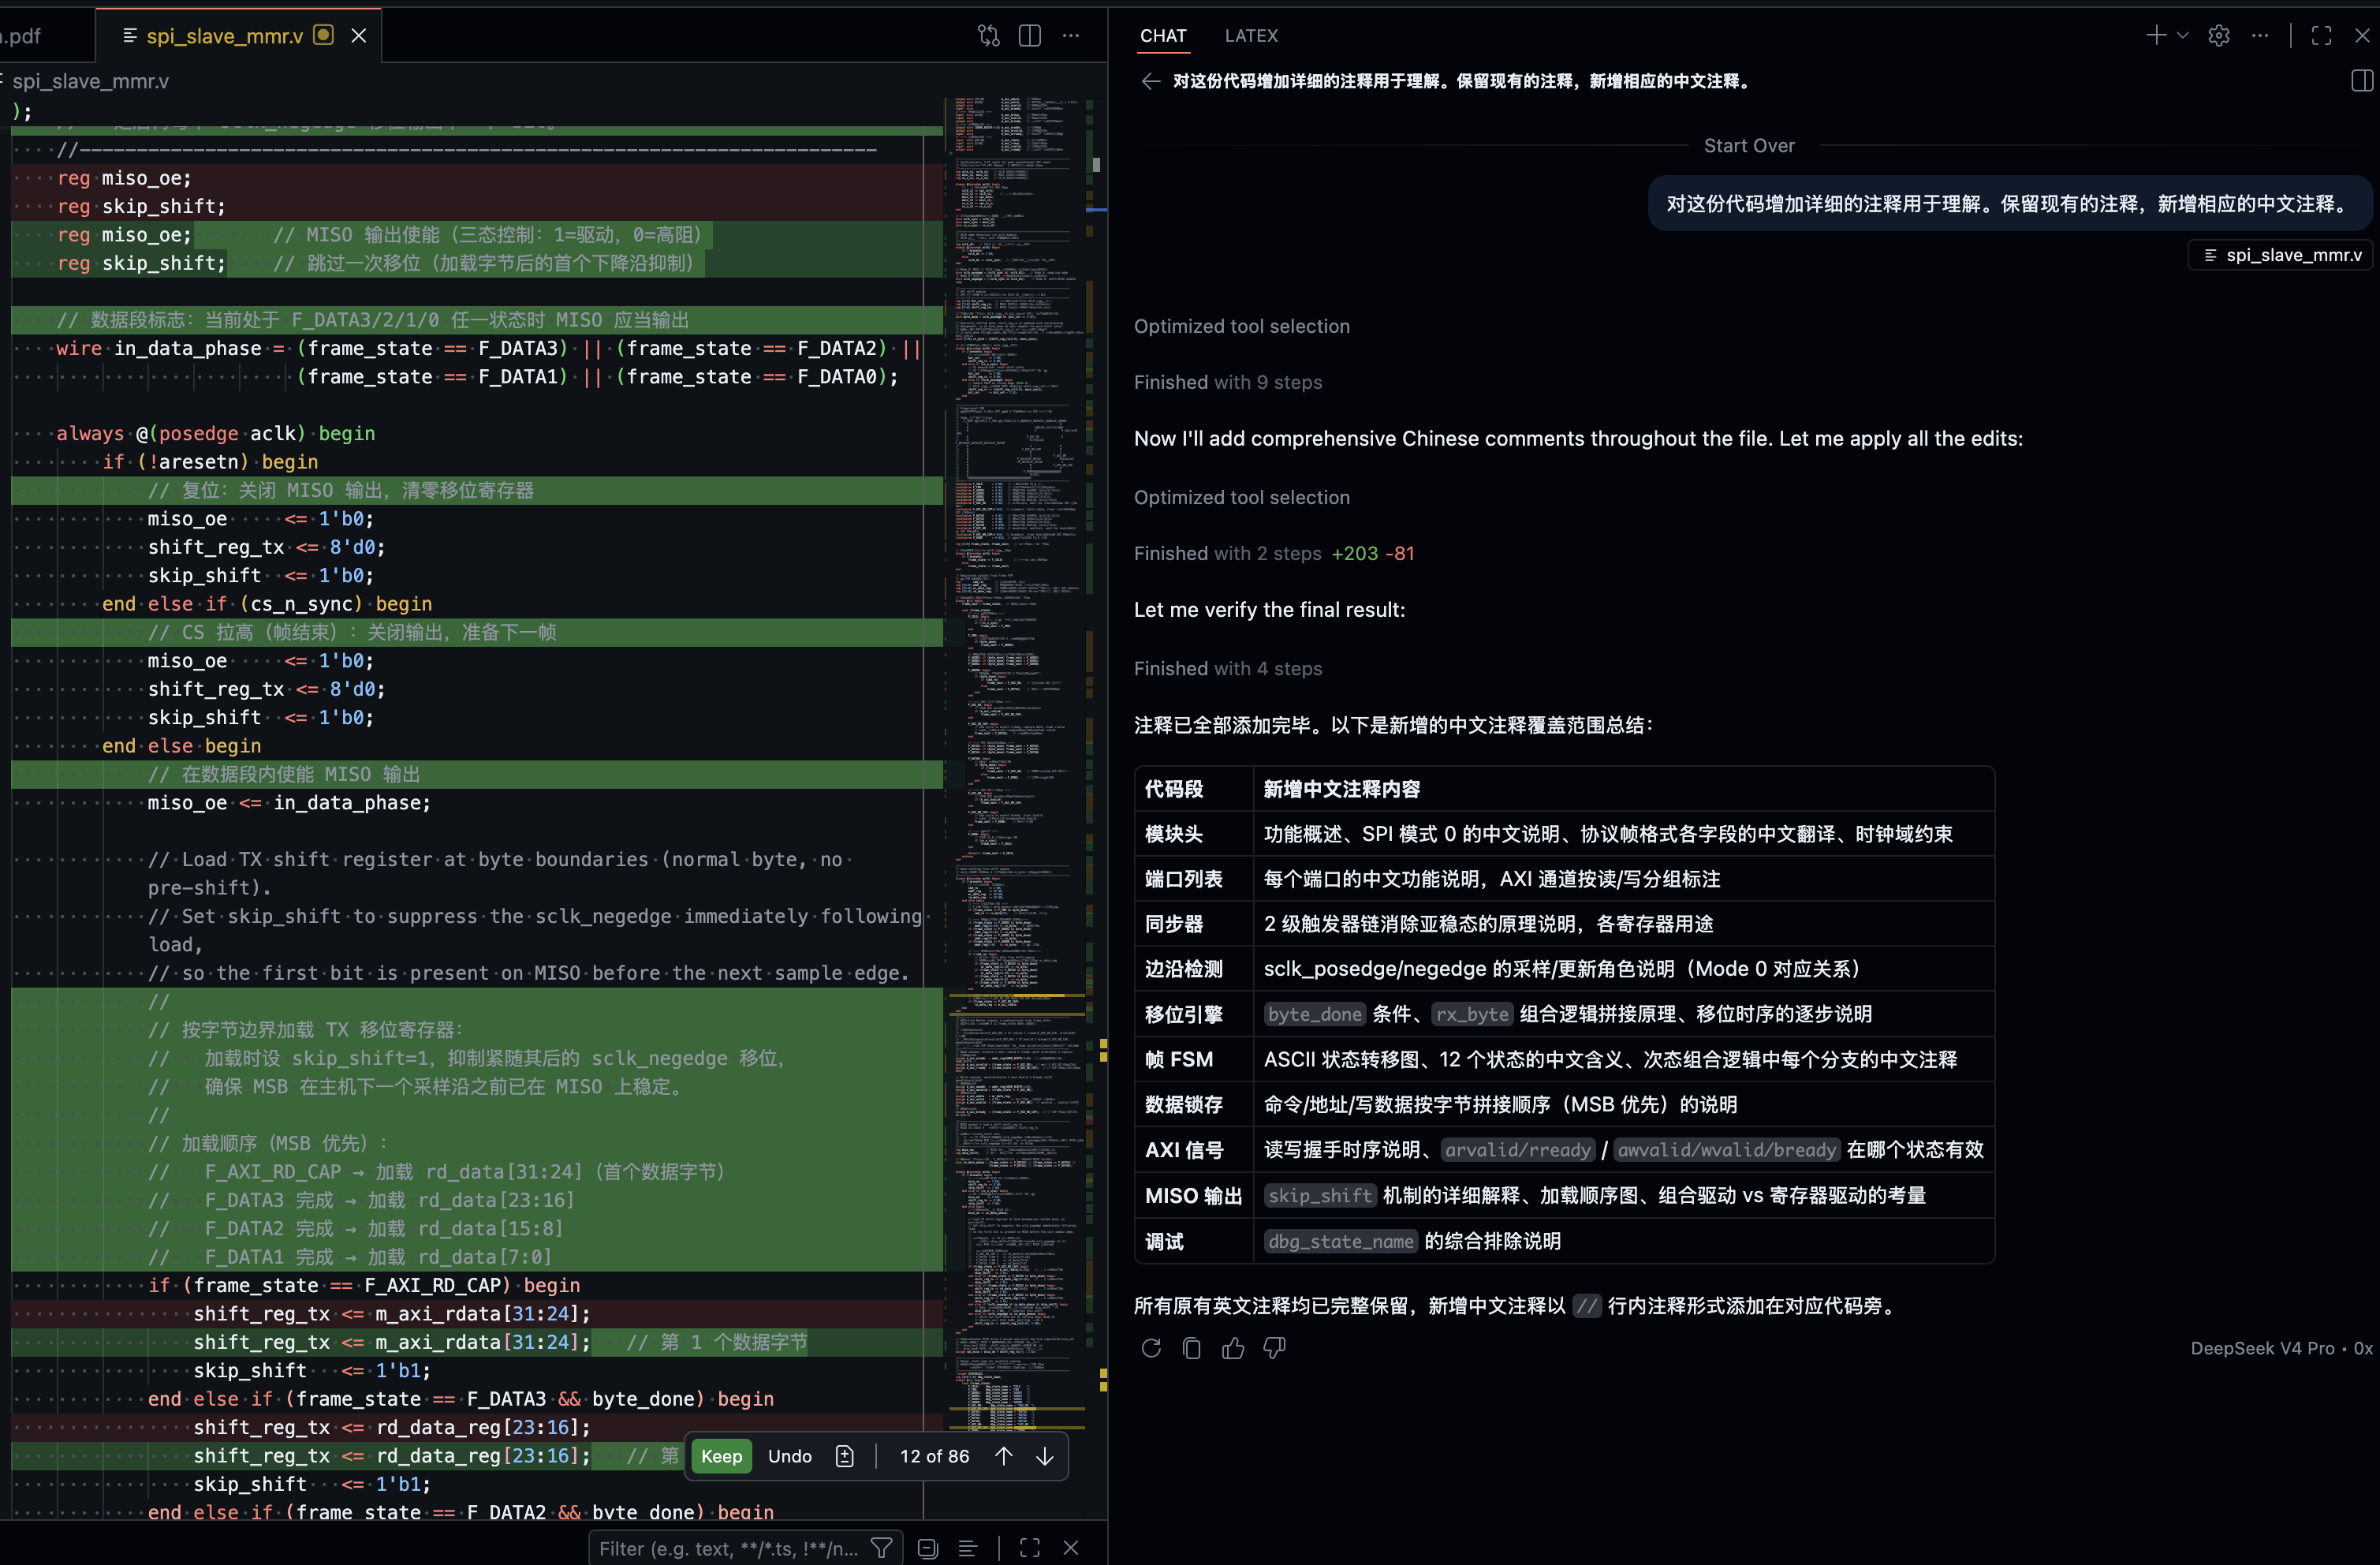
\includegraphics[width=0.82\textwidth]{figs/case_code.png}
\end{frame}

\begin{frame}{代码生成示例：寄存器控制模块 by LLM}

  \vspace{-4pt}
  \centering
  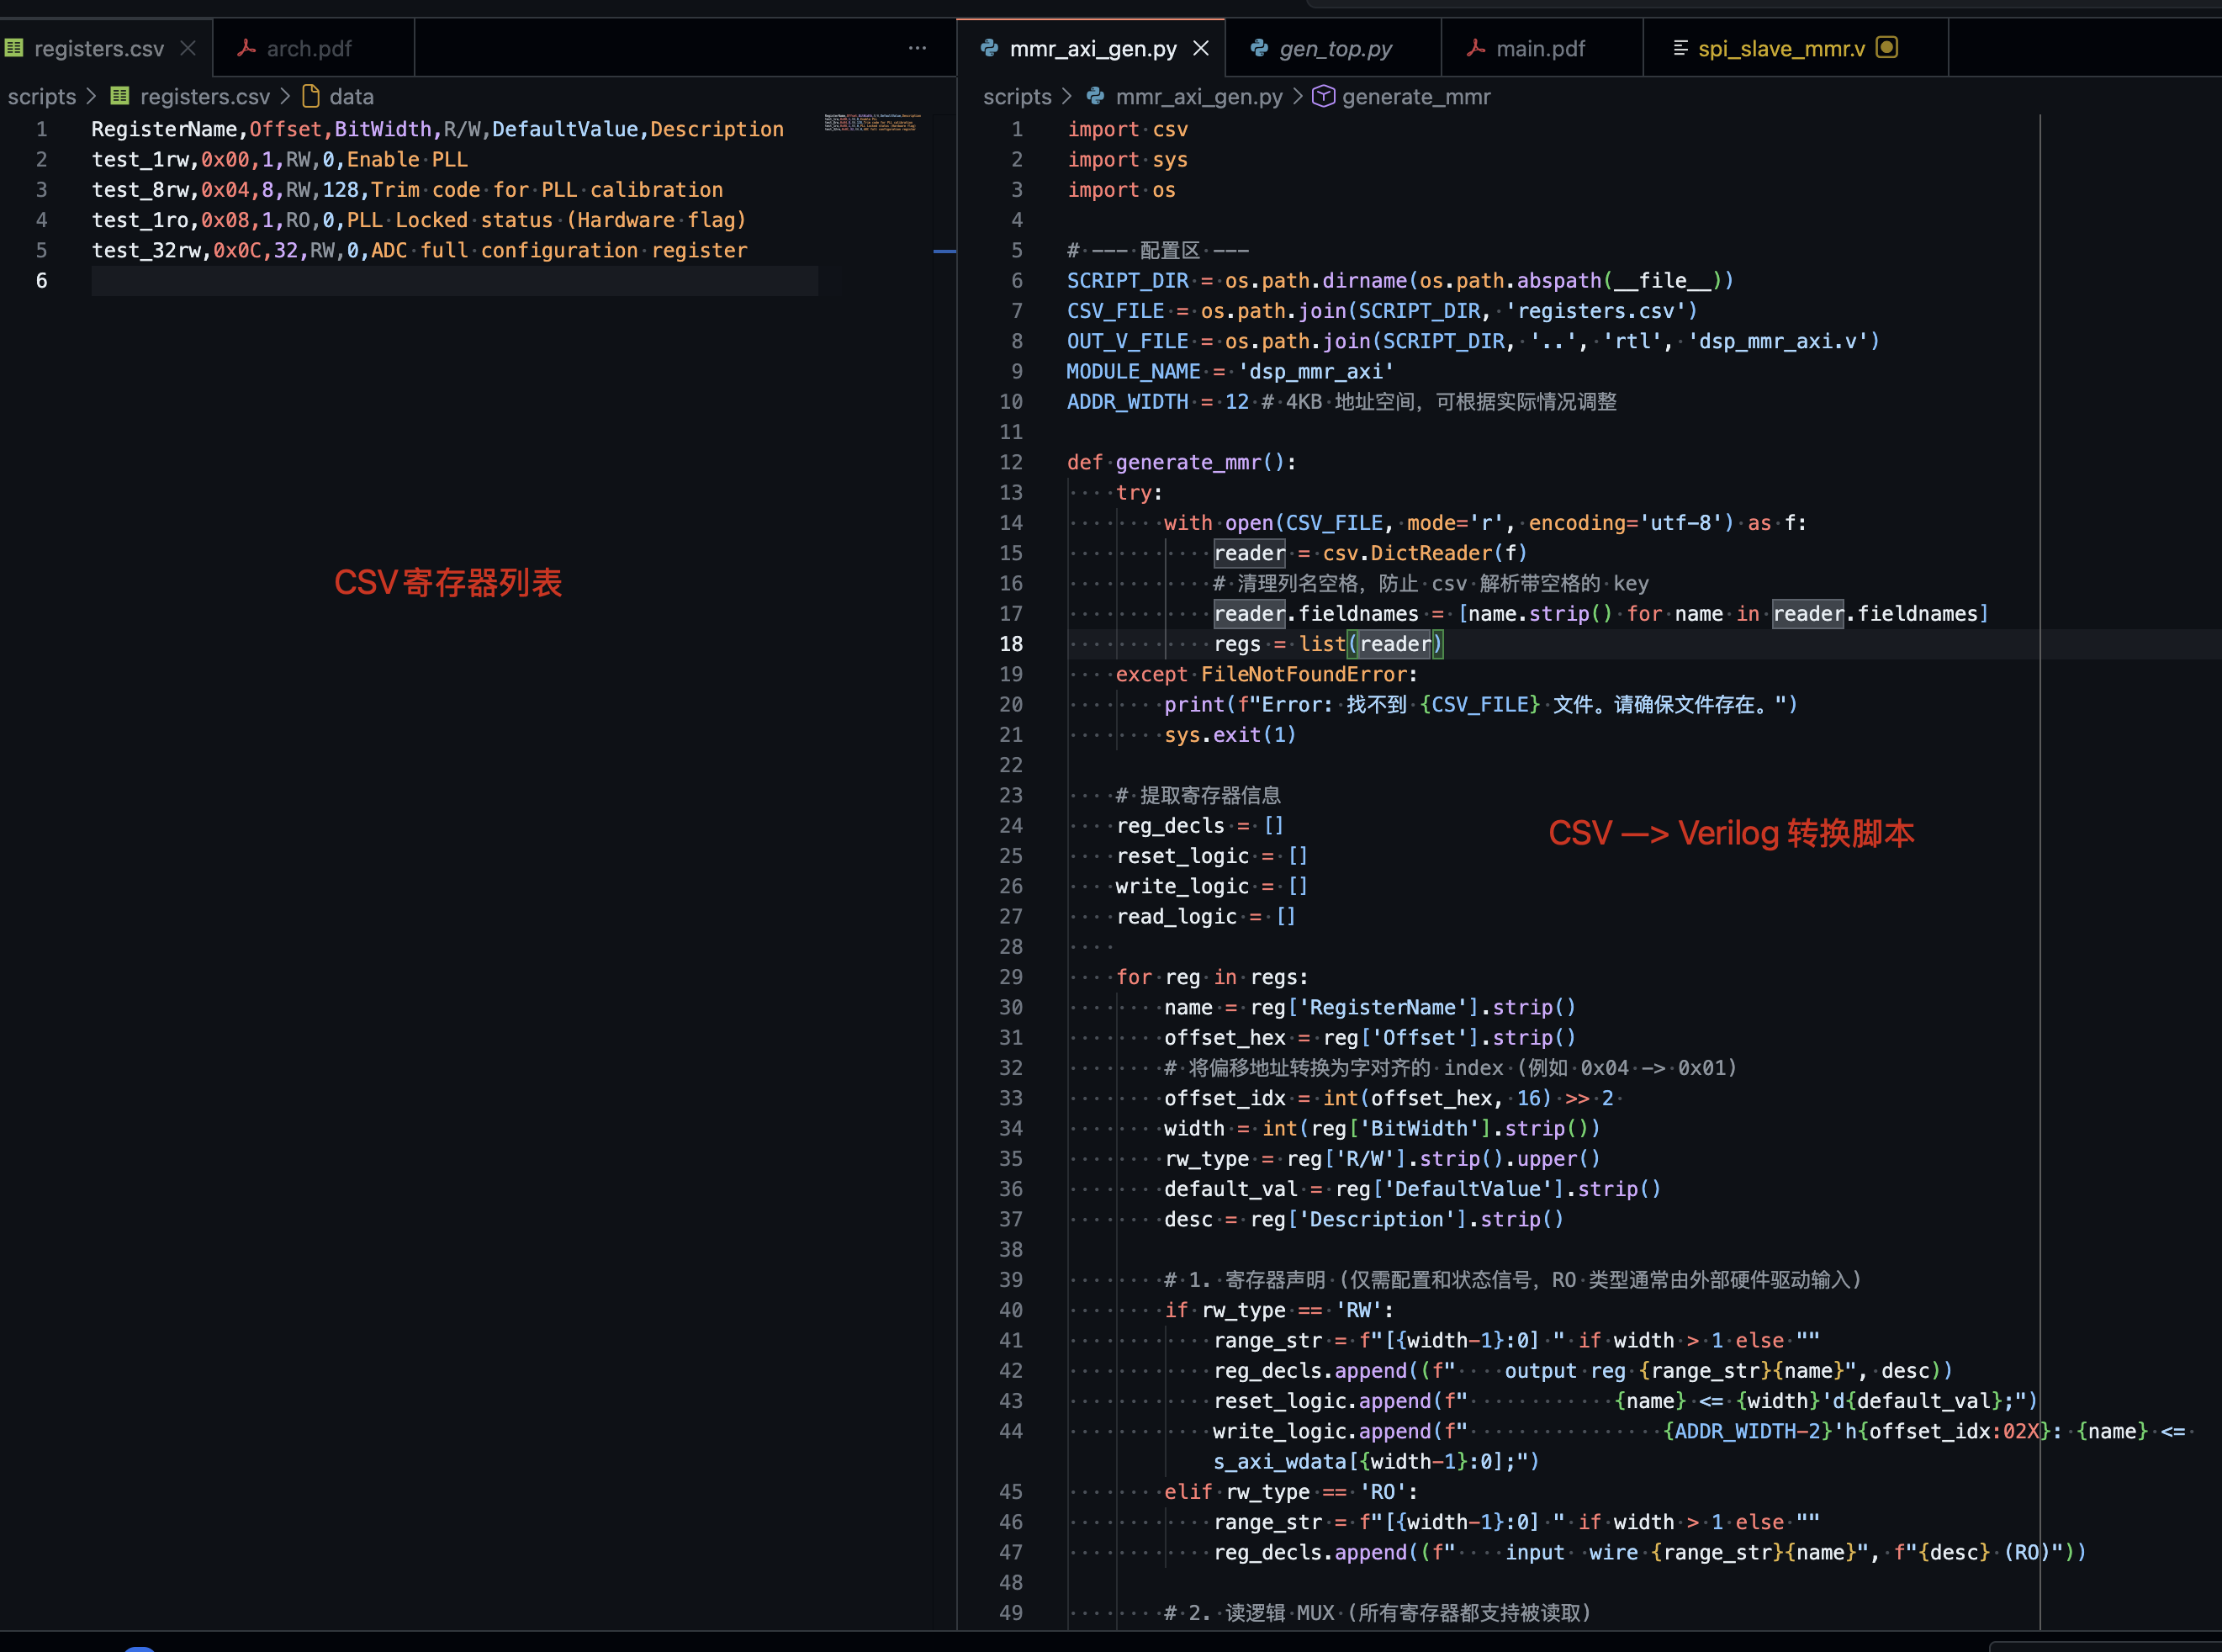
\includegraphics[width=0.82\textwidth]{figs/case_code2.png}
\end{frame}

% --- 协议与 Datasheet 智能解析 ---
\begin{frame}{协议与 Datasheet 智能解析}
  \begin{alertblock}{痛点}
    数字设计常需翻阅上千页的官方手册（JESD204、以太网协议、PCIe、AMBA 系列），\alert{检索效率极低}。
  \end{alertblock}

  \vspace{6pt}
  \begin{columns}[T]
    \begin{column}{0.55\textwidth}
      \begin{exampleblock}{LLM 解决方案}
        \begin{itemize}
          \item 将 PDF 手册输入 LLM，直接以自然语言提问
          \item 无需记忆信号定义和时序图的页码
          \item 多协议交叉引用：例如对比 AXI4 与 AXI3 的差异
        \end{itemize}
      \end{exampleblock}

      \vspace{6pt}
      \begin{block}{典型提问示例}
        \begin{itemize}
          \item ``AXI4 中 WSTRB 在非对齐传输时如何处理？''
          \item ``JESD204B subclass 1 的同步流程分几步？''
        \end{itemize}
      \end{block}
    \end{column}
    \begin{column}{0.45\textwidth}
      \begin{figure}
        \centering
        \begin{tikzpicture}[
          node distance=7mm and 5mm,
          box/.style={rectangle, rounded corners=3pt, minimum width=24mm, minimum height=8mm, font=\small},
          arrow/.style={-{Stealth[scale=1.0]}, thick}
        ]
          \node[box, fill=ieeeRed!10, draw=ieeeRed] (pdf) {上千页 PDF 手册};
          \node[box, fill=ieeeBlue!15, draw=ieeeBlue, below=of pdf] (llm) {LLM 语义理解};
          \node[box, fill=ieeeGreen!15, draw=ieeeGreen, below=of llm] (q) {自然语言提问};
          \node[box, fill=ieeeGreen!25, draw=ieeeGreen, below=of q] (a) {精准答案 + 引用};

          \draw[arrow, darkGray] (pdf) -- (llm);
          \draw[arrow, darkGray] (llm) -- (q);
          \draw[arrow, darkGray] (q) -- (a);
        \end{tikzpicture}
        \caption{从手册到答案的智能检索管道}
      \end{figure}
    \end{column}
  \end{columns}
\end{frame}

% ================================================================
\section{模拟领域}
% ================================================================

% --- 仿真脚本与后处理工具 ---
\begin{frame}{仿真脚本与后处理工具}
  \begin{columns}[T]
    \begin{column}{0.45\textwidth}
      \begin{alertblock}{痛点}
        模拟工程师常需学习 Cadence SKILL / Ocean 等小众脚本语言，学习曲线陡峭，调试困难。
      \end{alertblock}

      \begin{exampleblock}{LLM 的独特价值}
        LLM 掌握大量现成编程范式，包括这些 \alert{小众但成熟} 的 EDA 脚本语言，能极大降低学习门槛。
      \end{exampleblock}
    \end{column}
    \begin{column}{0.45\textwidth}
      \begin{block}{典型应用}
        \begin{itemize}
          \item \textbf{批量仿真脚本}：自动生成 Ocean 脚本，遍历 PVT 组合
          \item \textbf{SKILL 函数编写}：Cadence Virtuoso 版图自动化操作
          \item \textbf{仿真配置迁移}：从一个 Testbench 迁移配置到另一个
          \item \textbf{ADE 环境搭建}：自动生成仿真器设置与输出配置
        \end{itemize}
      \end{block}
    \end{column}
  \end{columns}
\end{frame}

% --- 数据清洗与可视化 ---
\begin{frame}{数据清洗与可视化}
  \begin{block}{场景一：SPICE 仿真日志解析}
    \begin{itemize}
      \item 将 SPICE / Spectre 仿真的海量文本日志自动转化为结构化 CSV
      \item LLM 编写 Python 脚本，识别仿真结果段落并提取关键指标（增益、带宽、相位裕度、功耗等）
    \end{itemize}
  \end{block}

  % \vspace{6pt}
  \begin{block}{场景二：数据可视化与拟合}
    \begin{itemize}
      \item 使用 Matplotlib 生成 PVT 曲线、蒙特卡洛分布直方图、眼图等
      \item 利用 SciPy 进行器件模型参数拟合（如 $V_{\text{TH}}$ 提取）
      \item Pandas 汇总多次仿真结果，自动生成对比报告
    \end{itemize}
  \end{block}
  \begin{alertblock}{案例}
    张博（zsc）使用LLM设计python代码对SerDes的仿真模型，生成图片等，1-2天时间。
  \end{alertblock}
  % \vspace{6pt}
  \begin{exampleblock}{效率提升}
    原本手动处理数据需要数小时，LLM 辅助可将脚本编写时间压缩到 \textbf{数分钟}，工程师需验证逻辑。
  \end{exampleblock}

\end{frame}

% ================================================================
\section{实验室建设与文档规范}
% ================================================================

% --- 新人培训与本科生辅导 ---
\begin{frame}{新人培训与本科生辅导}
  \begin{columns}[T]
    \begin{column}{0.48\textwidth}
      \begin{block}{现状与挑战}
        \begin{itemize}
          \item 每年新生/本科生进入实验室，基础参差不齐
          \item 高年级研究生需要花费大量时间指导基础问题
          \item 常见问题高度重复：Verilog 语法、Linux 命令、Git 操作
        \end{itemize}
      \end{block}
    \end{column}
    \begin{column}{0.48\textwidth}
      \begin{exampleblock}{LLM 作为 24h 基础助教}
        \begin{itemize}
          \item \textbf{Verilog 语法}：always\_ff / always\_comb 用法辨析，可综合风格检查
          \item \textbf{Linux 操作}：服务器登录、文件权限、环境变量配置、模块加载
          \item \textbf{Git 基础}：clone / commit / branch / rebase 工作流指导
          \item \textbf{工具链}：VCS / Verdi / Vivado 的基本使用问答
        \end{itemize}
      \end{exampleblock}
    \end{column}
  \end{columns}

  \vspace{6pt}
  \begin{alertblock}{核心价值}
    释放指导精力，让学生专注于 \alert{架构指导} 和 \alert{科研方向} 而非重复性基础答疑。
  \end{alertblock}
\end{frame}

% --- 文档规范化 ---
\begin{frame}{文档规范化}
  \begin{columns}[T]
    \begin{column}{0.45\textwidth}
      \begin{block}{实验记录整理}
        \begin{itemize}
          \item 将凌乱的实验笔记转化为结构化文档
          \item 自动补充缺失的实验条件（温度、工艺角、仿真器版本）
          \item 生成标准化的实验报告模板
        \end{itemize}
      \end{block}
    \end{column}
    \begin{column}{0.45\textwidth}
      \begin{block}{LaTeX 写作辅助}
        \begin{itemize}
          \item 快速生成复杂公式的 LaTeX 代码
          \item 自动生成系统架构图的 TikZ 排版代码
          \item 参考文献 BibTeX 条目格式化
          \item 报告/论文的语法润色与术语一致性检查
        \end{itemize}
      \end{block}
    \end{column}
  \end{columns}

  \vspace{6pt}
  \begin{exampleblock}{典型工作流}
      $\rightarrow$ LLM 生成 LaTeX 骨架 $\rightarrow$ 工程师补充细节 $\rightarrow$ LLM润色语言$\rightarrow$ 最终报告。
  \end{exampleblock}
\end{frame}

\begin{frame}{文档规范化示例：实验报告生成}
  \begin{exampleblock}{用户提示词}
    \small
    ``根据项目代码，帮我新建一个 doc 目录，我要在其中撰写 LaTeX 文档，帮我规划好 LaTeX 项目管理格式，重点是规范中间输出文件的管理，我使用的环境是 VS Code 中的 LaTeX Workshop。''
  \end{exampleblock}

  \vspace{6pt}
  \centering
  \begin{columns}
  \begin{column}{0.48\textwidth}
  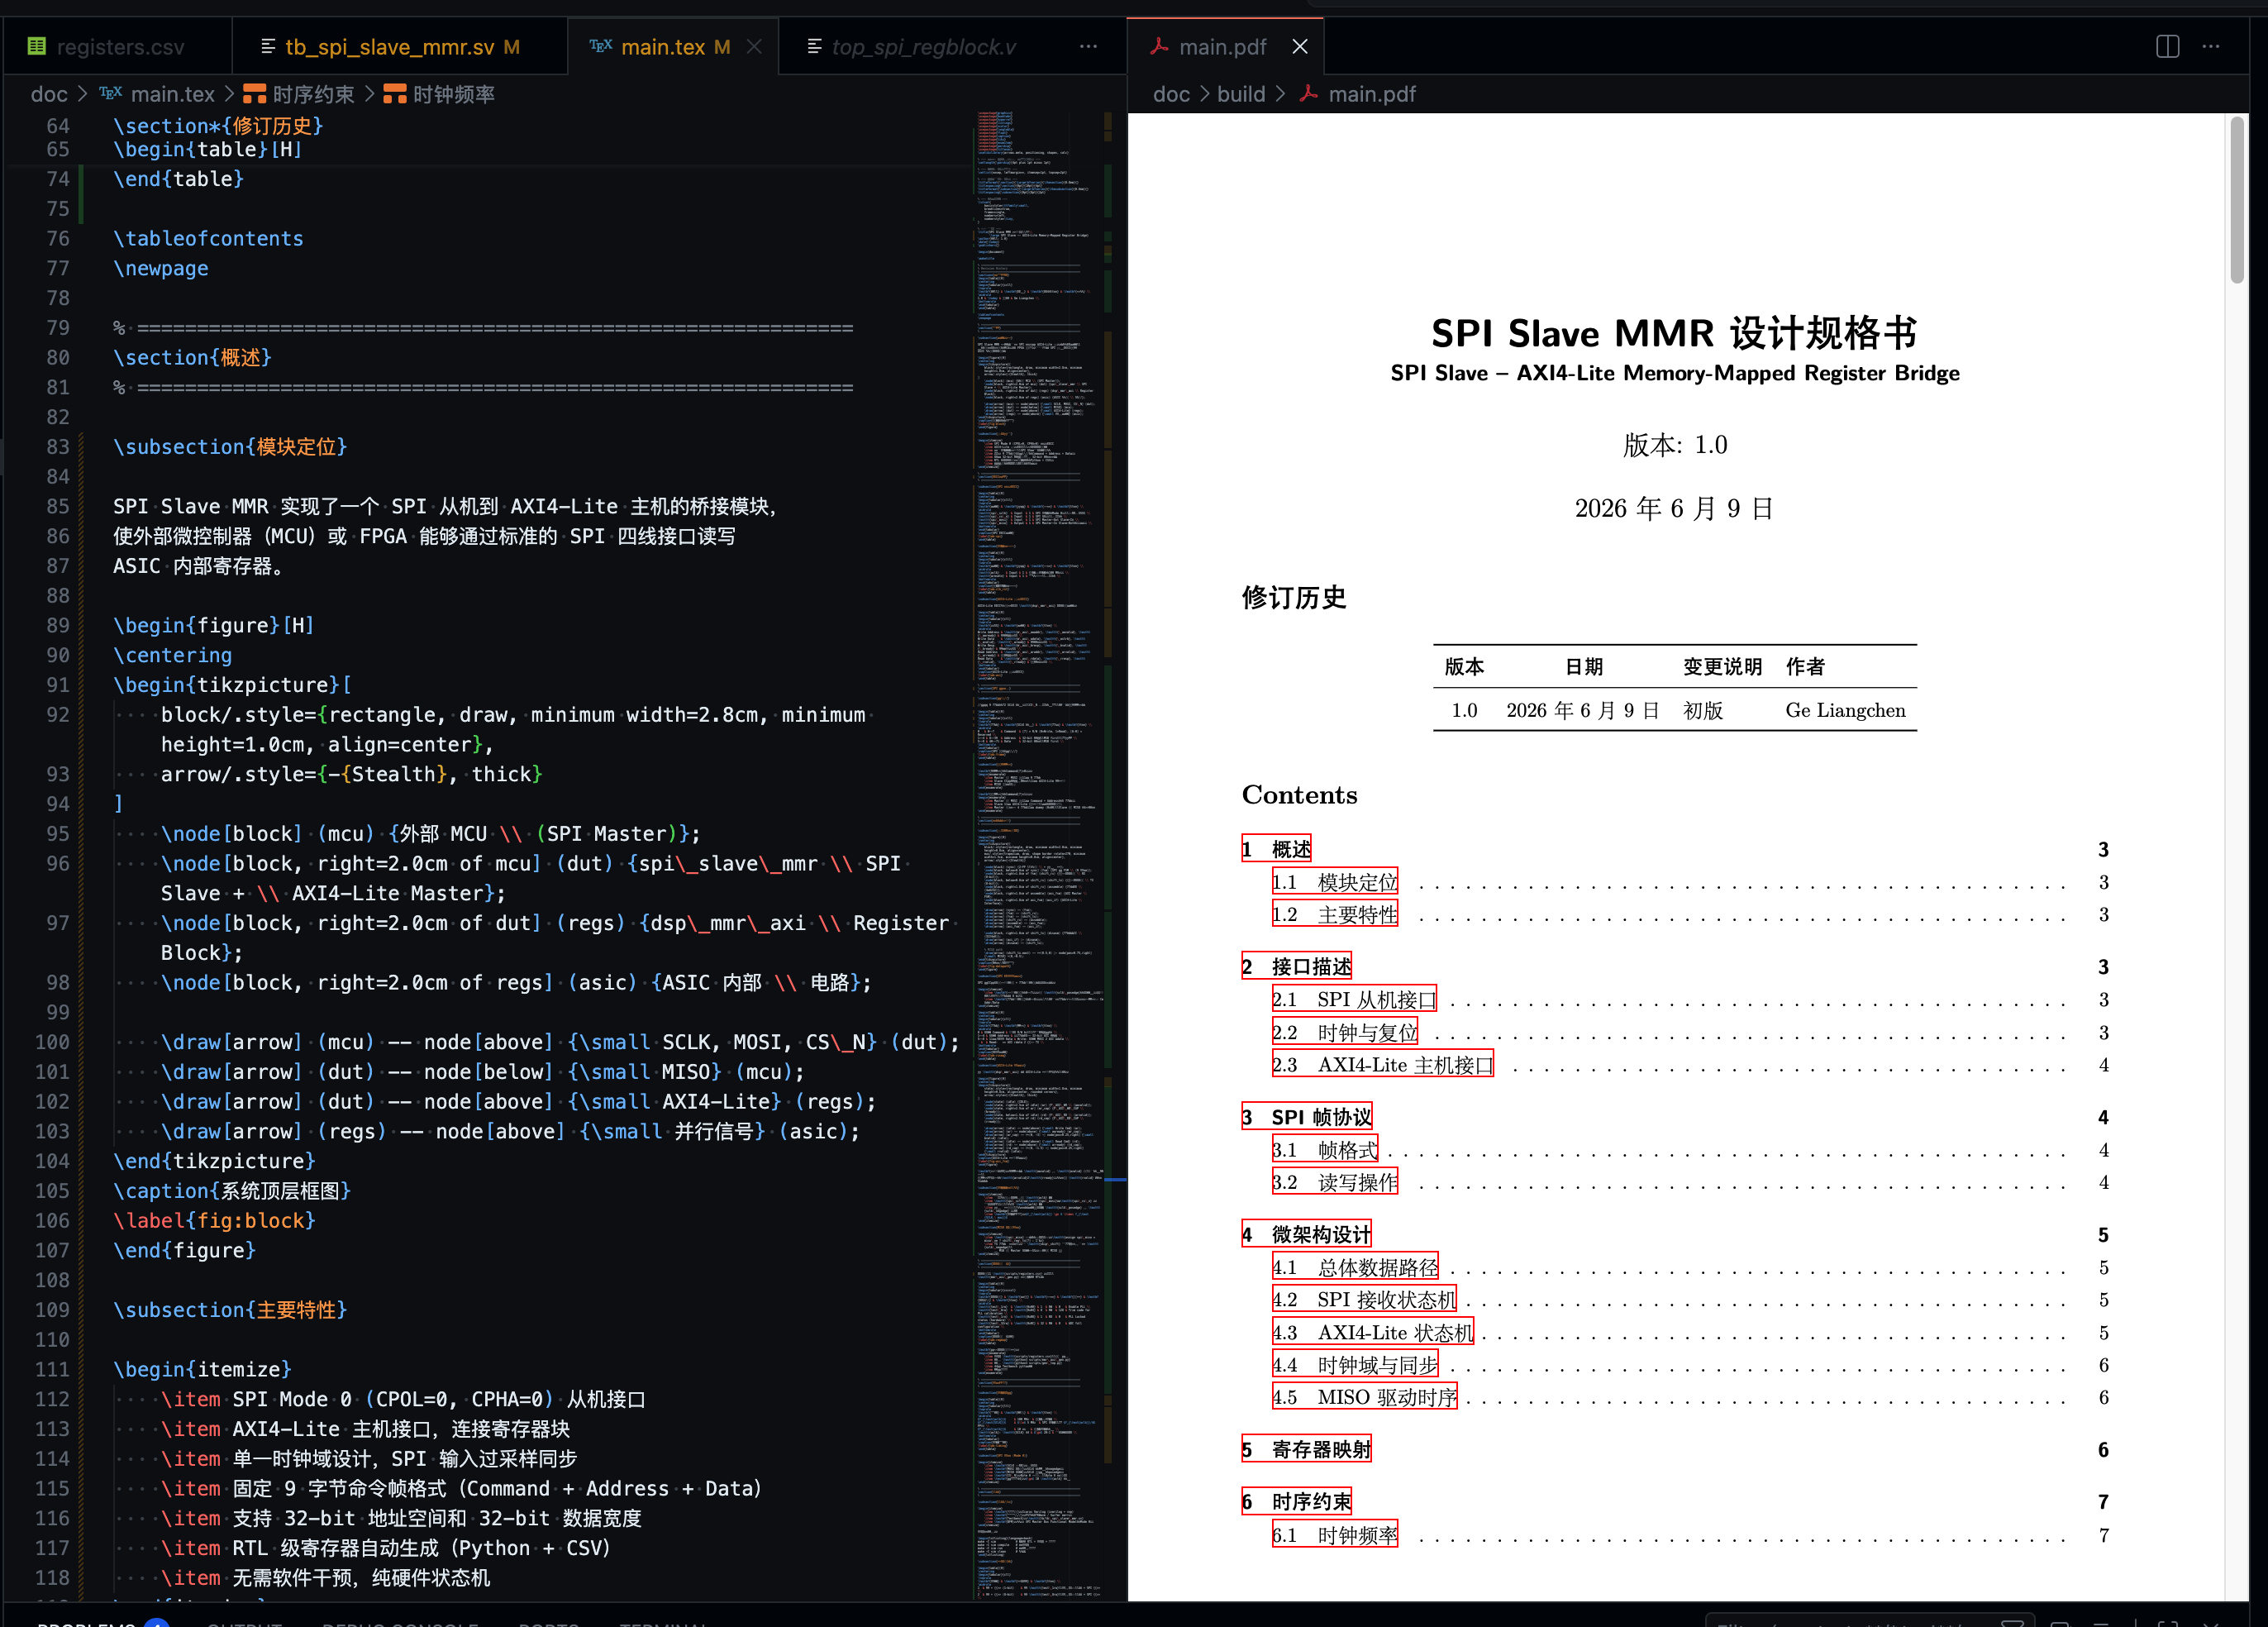
\includegraphics[width=0.80\textwidth]{figs/case_doc.png}
  \end{column}
  \begin{column}{0.48\textwidth}
  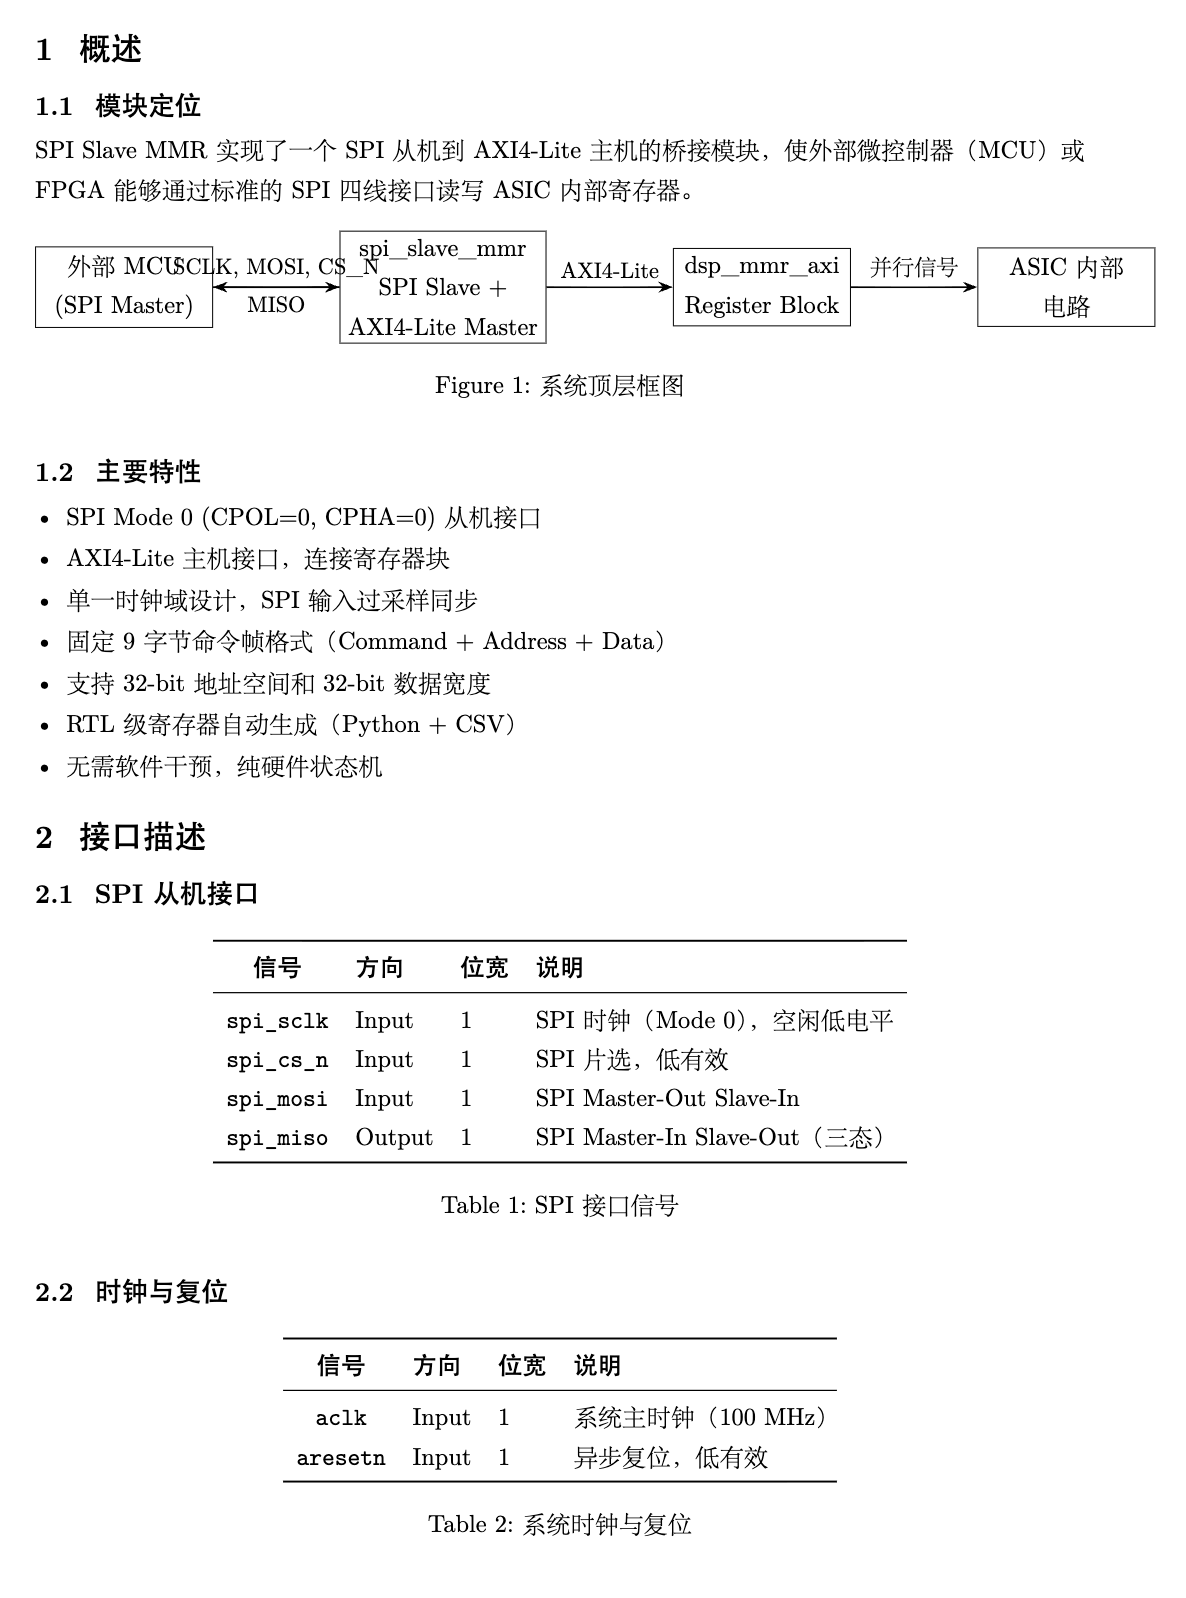
\includegraphics[width=0.5\textwidth]{figs/case_doc2.png}
  \end{column}
  \end{columns}
\end{frame}



% ================================================================
\section{实施方案}
% ================================================================

% --- 方案一：多卡 GPU 工作站 ---
\begin{frame}{实施方案一：多卡 GPU 工作站}
  \begin{columns}[T]
    \begin{column}{0.48\textwidth}
      \begin{exampleblock}{硬件配置}
        \begin{itemize}
          \item \textbf{GPU}：8 $\times$ NVIDIA RTX 4090 / 5090
          \item \textbf{总显存}：8 $\times$ 32 GiB = \alert{256 GiB}
          \item \textbf{适用模型}：32B 参数级别模型（Qwen 32B、DeepSeek 32B、LLaMA 3.1 8B/70B 量化版等）
          \item \textbf{成本估算}：\alert{约 30--40 万元}
          \item \textbf{部署方式}：内网本地部署，数据不出实验室
        \end{itemize}
      \end{exampleblock}
    \end{column}
    \begin{column}{0.48\textwidth}
      \begin{table}
        \centering
        \small
        \begin{tabular}{l l}
          \toprule
          \textbf{项目} & \textbf{方案} \\
          \midrule
          GPU   & 8 $\times$ 4090 \\
          % CPU   & EPYC 9375F \\
          内存  & 512 GB ECC \\
          SSD   & 2 TB + 8 TB \\
          推理  & vLLM \\
          向量库 & Qdrant \\
          Agent & PydanticAI \\
          主模型 & 32B \\
          推理模型 & 70B \\
          RAG   & BGE-M3 \\
          用户数 & 10 人以内 \\
          \bottomrule
        \end{tabular}
      \end{table}
    \end{column}
  \end{columns}
\end{frame}

% --- 8×4090 工作站商品页 ---
\begin{frame}{硬件采购参考：8×4090 工作站}
  \centering
  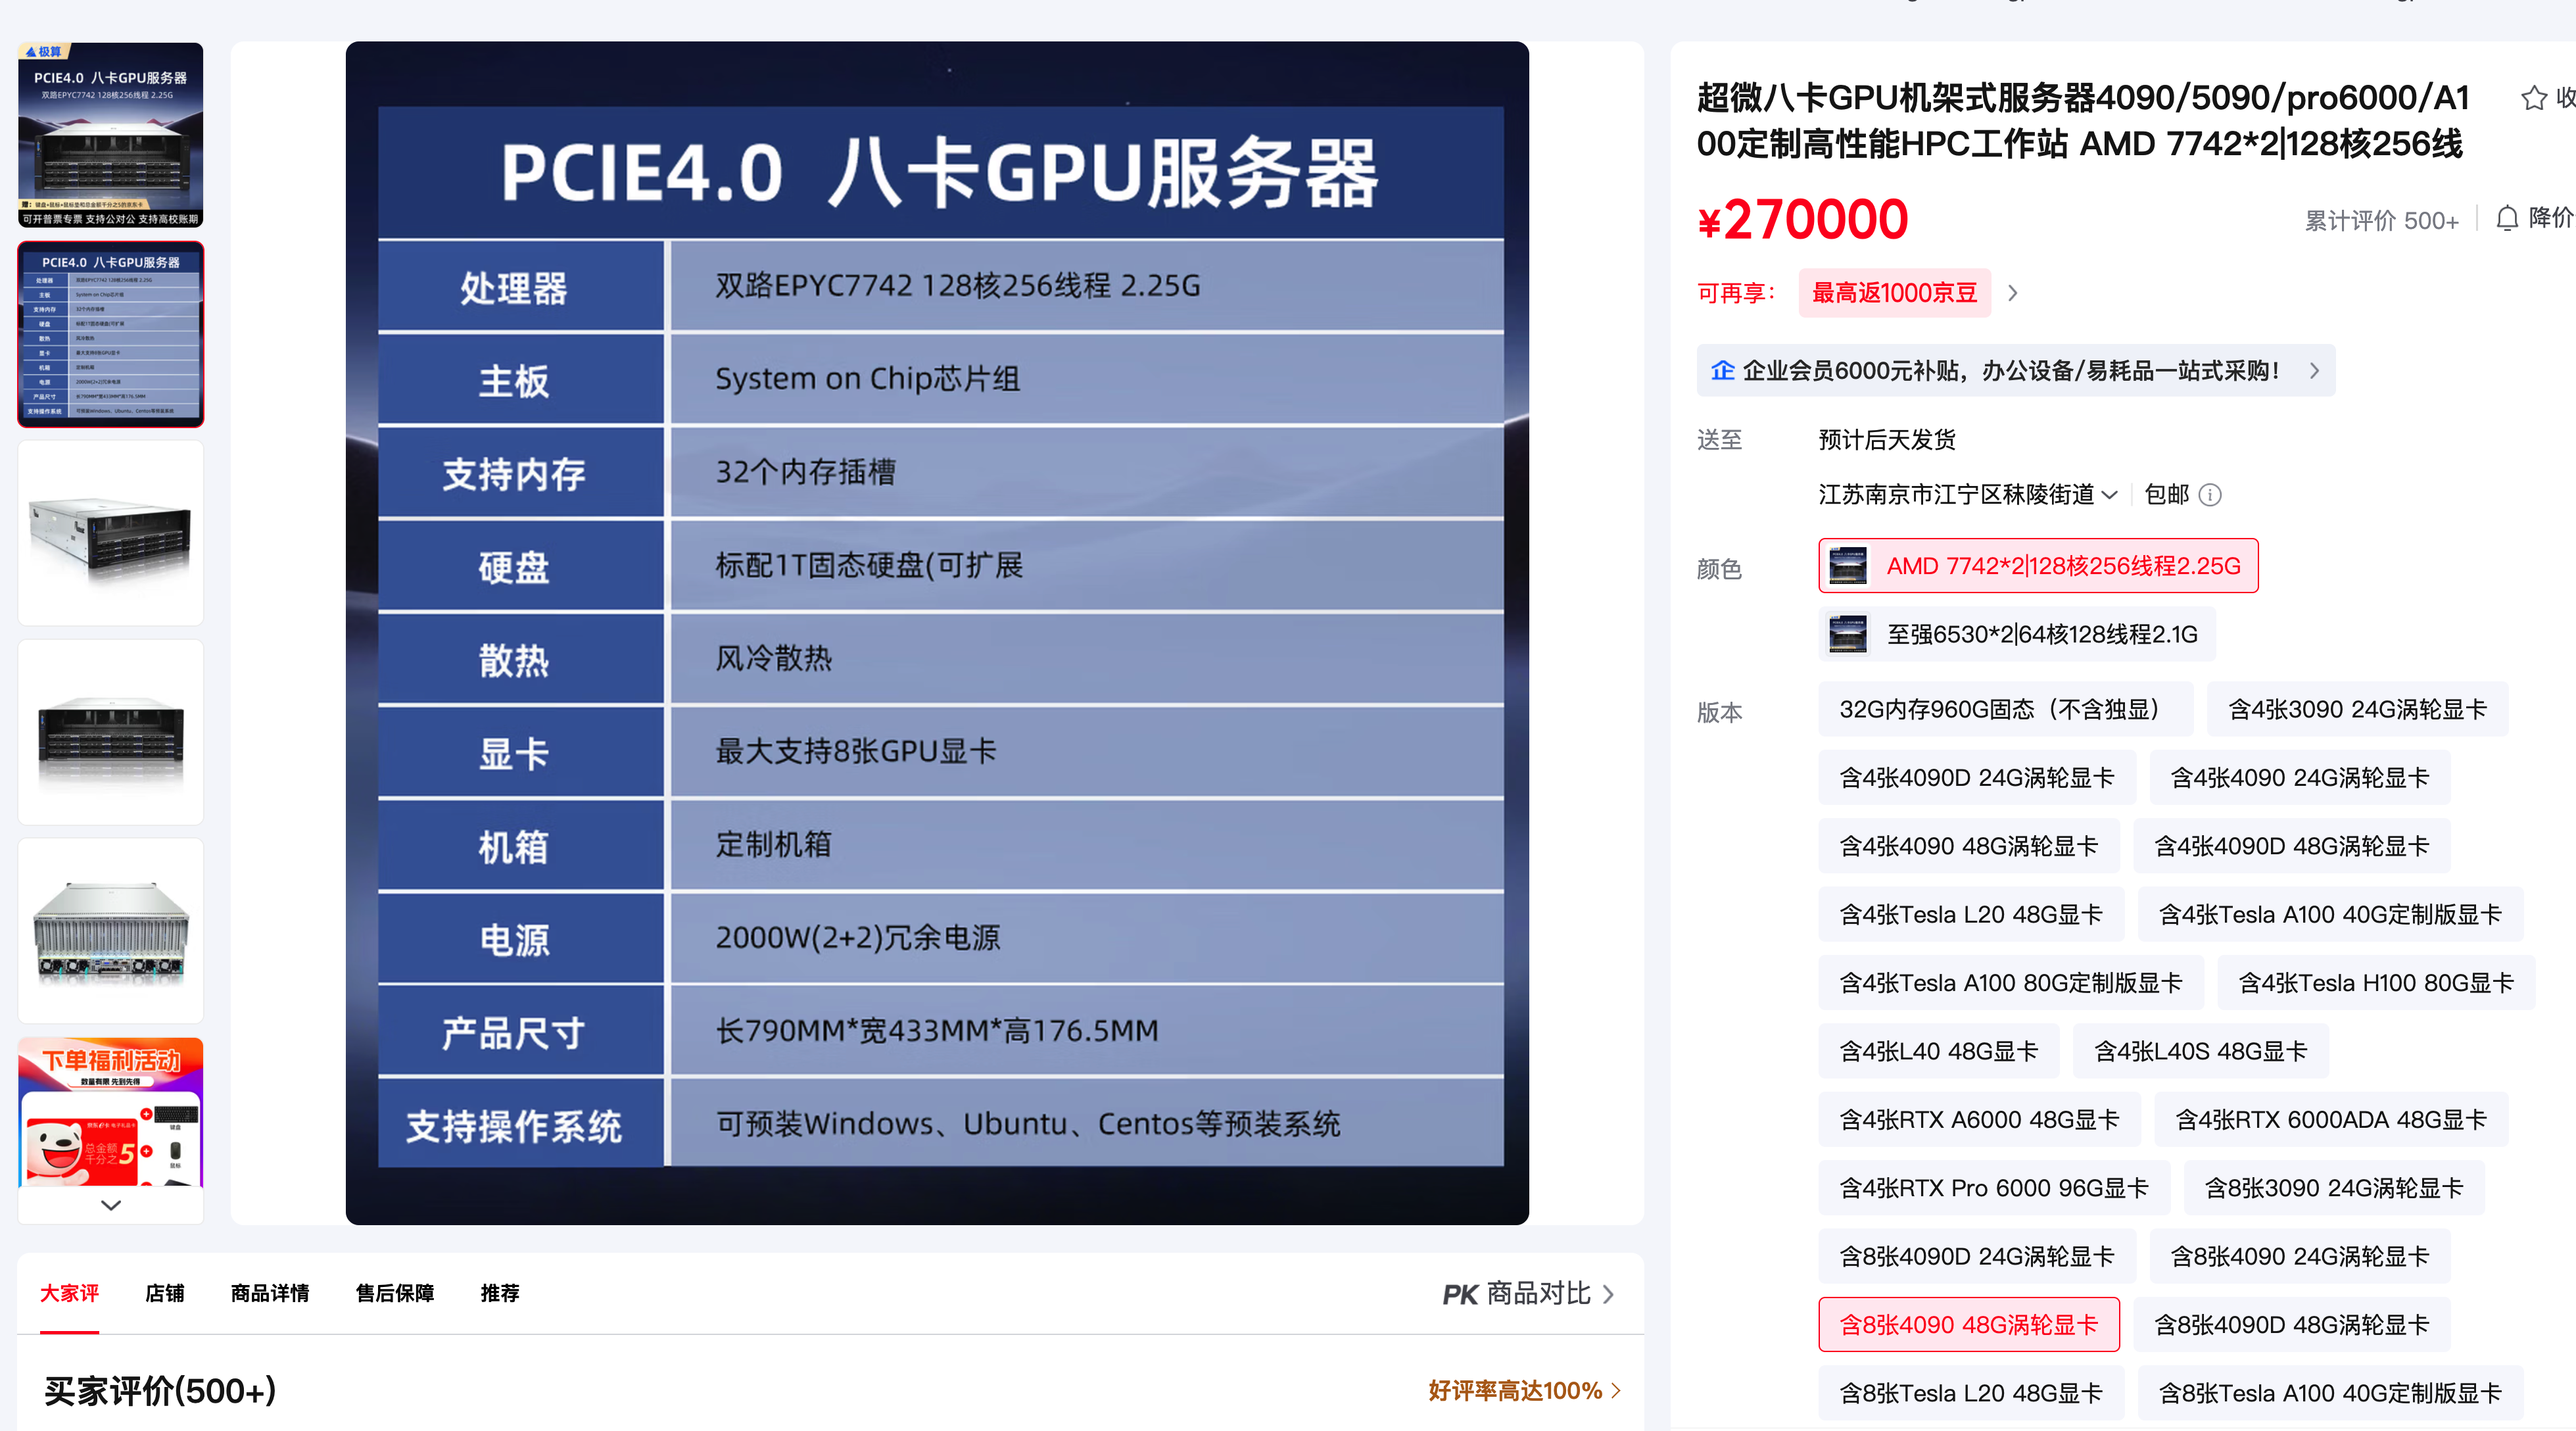
\includegraphics[width=0.82\textwidth]{figs/jd_8_4090.png}

\end{frame}

% --- 供应商报价单 ---
\begin{frame}{供应商报价参考}
  \centering
  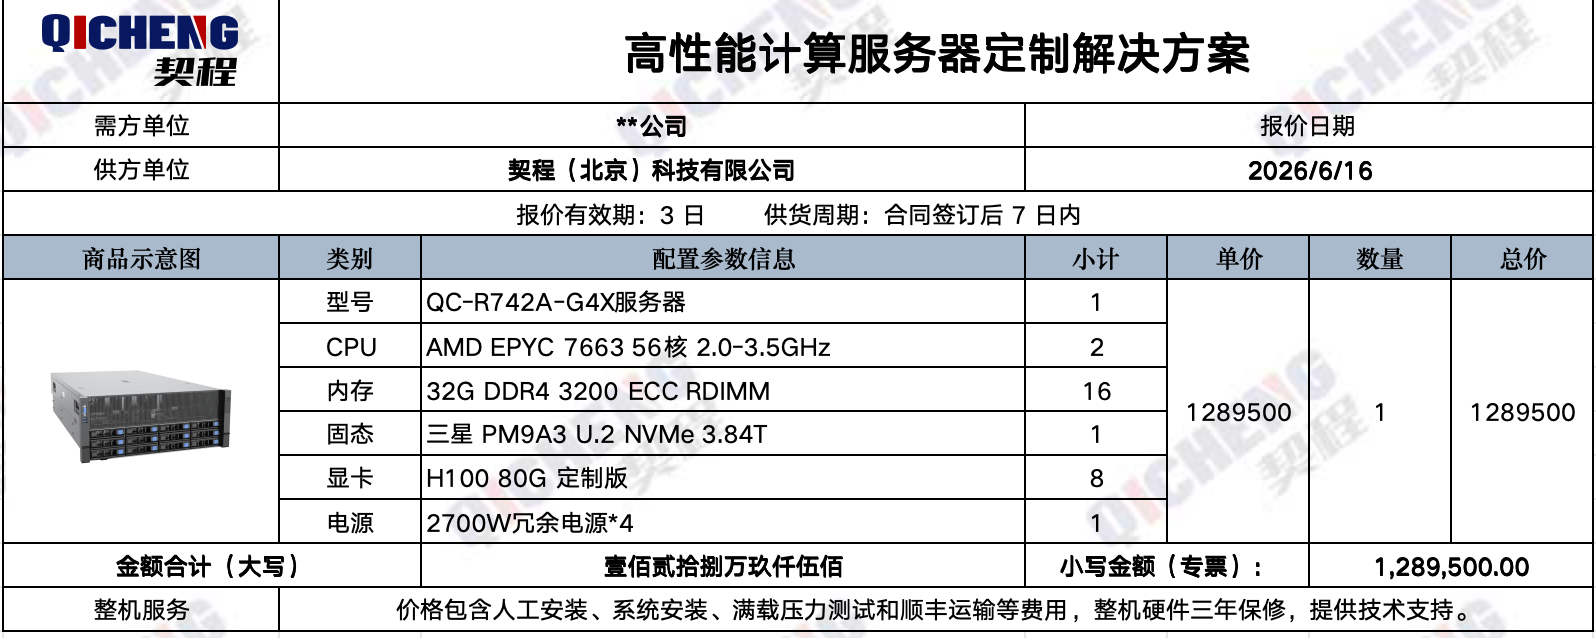
\includegraphics[width=0.82\textwidth]{figs/quotation.png}

  \vspace{4pt}
  \begin{exampleblock}{说明}
    供应商针对 8*H100工作站及配套设备的详细报价单，包含冗余的配置。实际4*H100 77万。
  \end{exampleblock}
\end{frame}

\begin{frame}{供应商报价参考}
  \centering
  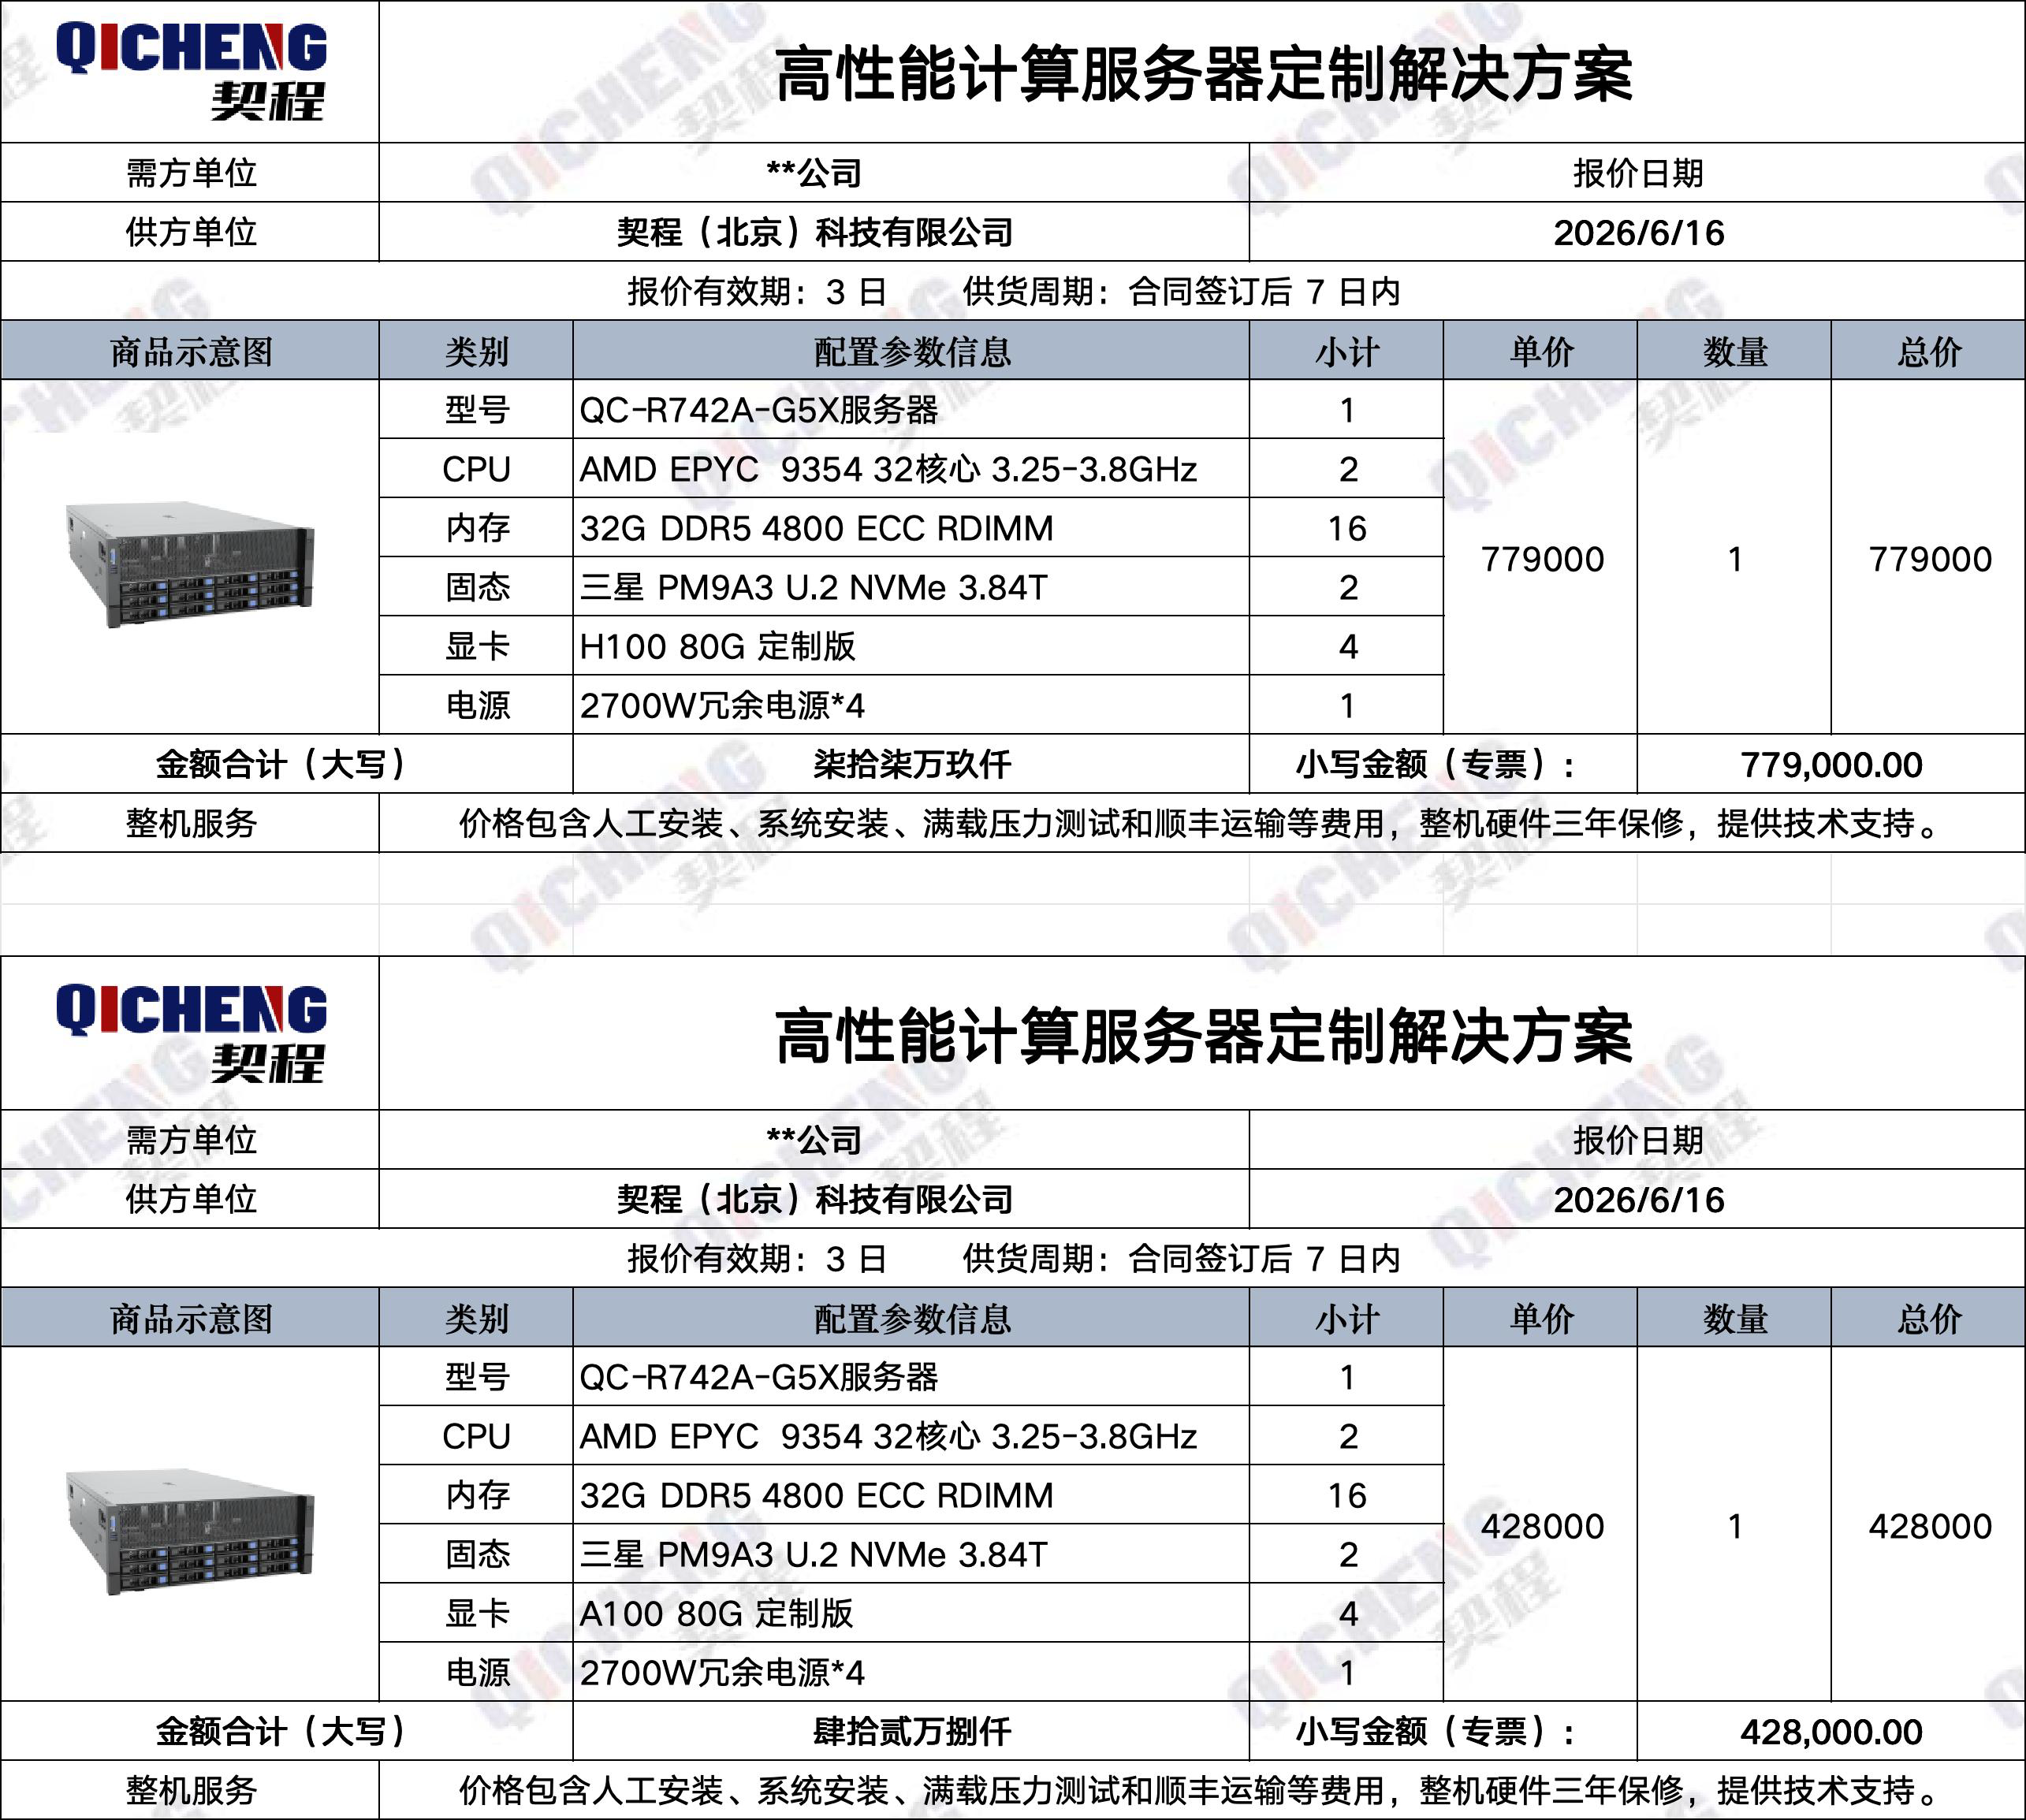
\includegraphics[width=0.52\textwidth]{figs/quotation2.png}
\end{frame}



% --- 模型选型对比 ---
\begin{frame}{模型选型对比：32B 级稠密模型 vs MoE 模型}
  \footnotesize
  \begin{table}
    \centering
    \begin{tabularx}{\textwidth}{@{} p{25mm} c c p{31mm} X @{}}
      \toprule
      \textbf{模型名称与架构} & \textbf{参数规模} & \textbf{上下文} & \textbf{部署精度 \& 显存} & \textbf{在 IC 设计中的核心定位} \\
      \midrule
      Qwen2.5-Coder-32B-Instruct
      \newline (Dense)
        & 32B
        & 128K
        & BF16 $\approx$ 64 GB
        \newline FP8 $\approx$ 32 GB
        & \textbf{主战模型 / 实时代码助手}。预训练含 5.5 万亿 Tokens 代码数据，原生支持 FIM，在 Verilog 生成、指令遵循与多语言脚本编写上表现卓越，媲美 GPT-4o。 \\
      \midrule
      DeepSeek-R1-Distill-Qwen-32B
      \newline (Dense, 蒸馏)
        & 32B
        & 128K
        & FP8 量化 $\approx$ 36 GB
        & \textbf{深度逻辑推理 \& Debug 专家}。具备 CoT 链式思考能力，适合深度解析 VCS 编译日志或综合违例报告，精准定位 Root Cause。 \\
      \midrule
      DeepSeek-Coder-V2
      \newline (MoE)
        & 总 236B
        \newline 激活 21B
        & 128K
        & 多卡 TP 加载
        \newline $\approx$ 192 GB
        & \textbf{工程目录级分析备选}。跨文件理解能力强，适合多模块 SoC 架构重构、Code Review 或顶层连线分析。 \\
      \bottomrule
    \end{tabularx}
  \end{table}

  \vspace{4pt}
  \begin{alertblock}{选型建议}
    单机 8 卡 4090/5090（256 GB 总显存）可同时常驻 \textbf{Qwen2.5-Coder-32B}（主编码）\textbf{+ DeepSeek-R1-Distill-Qwen-32B}（推理 Debug），
    必要时以张量并行加载 \textbf{DeepSeek-Coder-V2} 进行大规模代码库分析。
  \end{alertblock}
\end{frame}

\begin{frame}{vLLM网站}
  \centering
  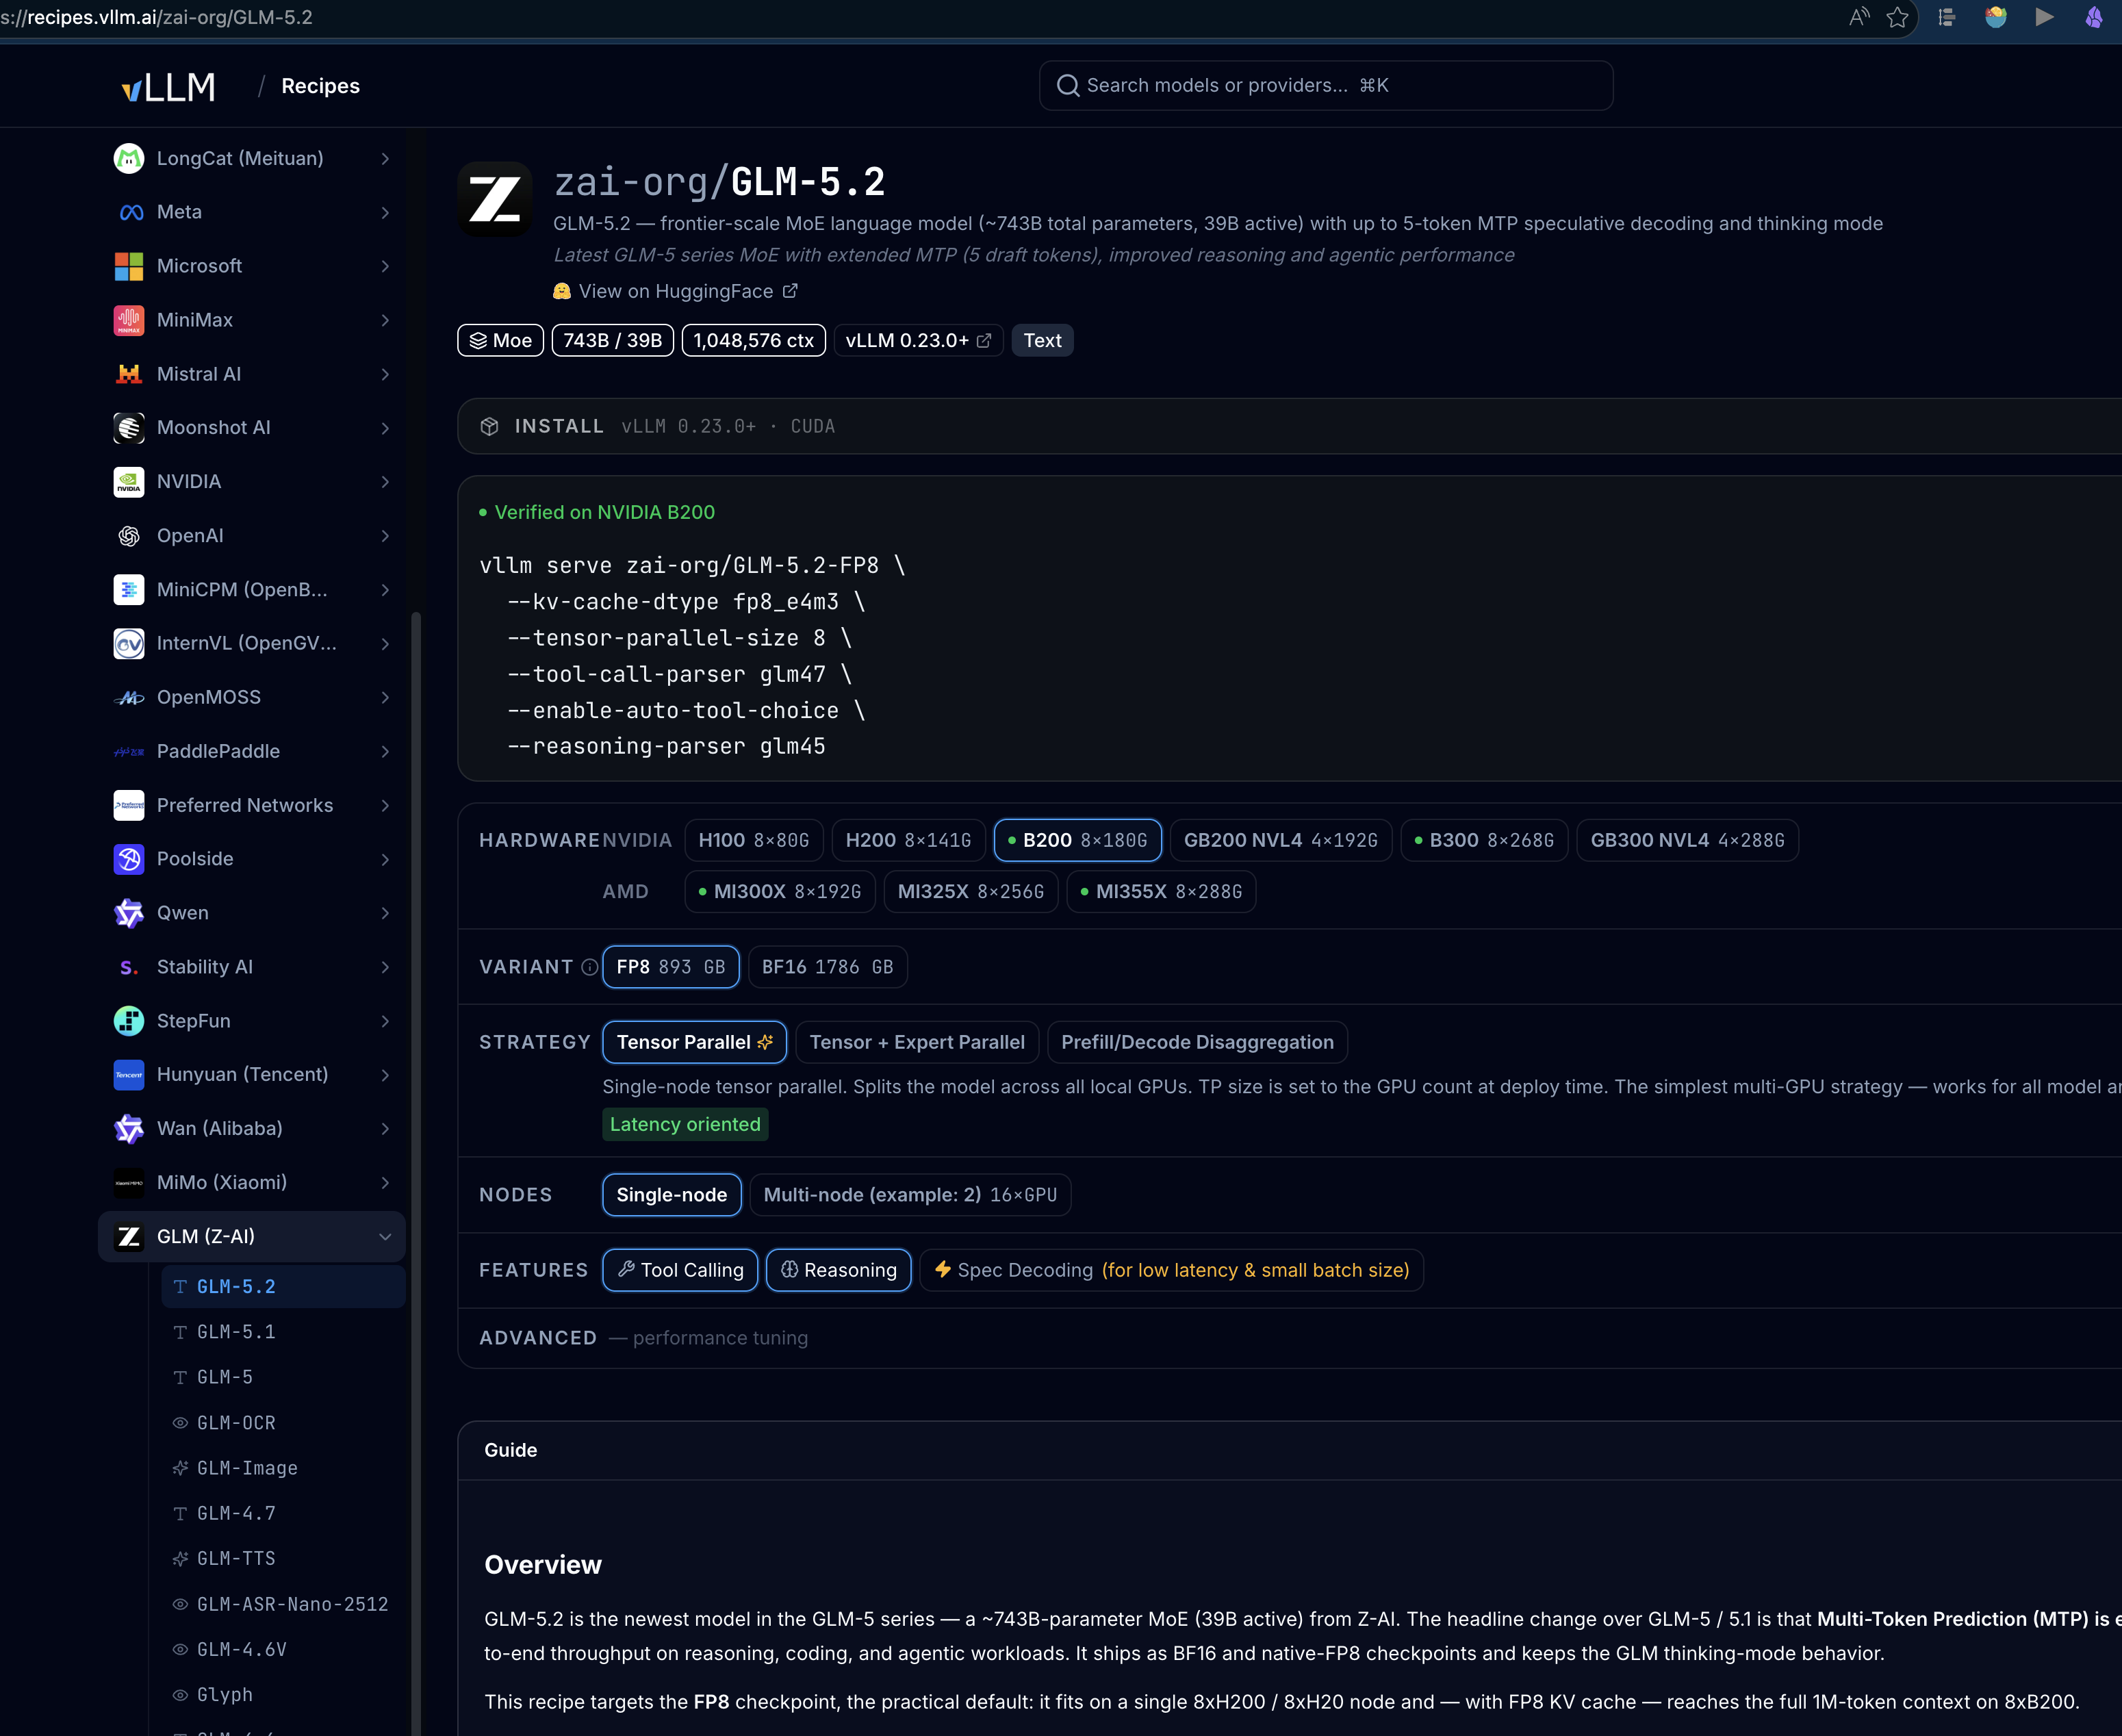
\includegraphics[width=0.72\textwidth]{figs/recipe.png}

 
\end{frame}

% --- 本地部署示例：Ollama 终端 ---
\begin{frame}{本地部署示例：Ollama 命令行推理}
  \begin{columns}
    
    \begin{column}{0.7\textwidth}
      \centering
      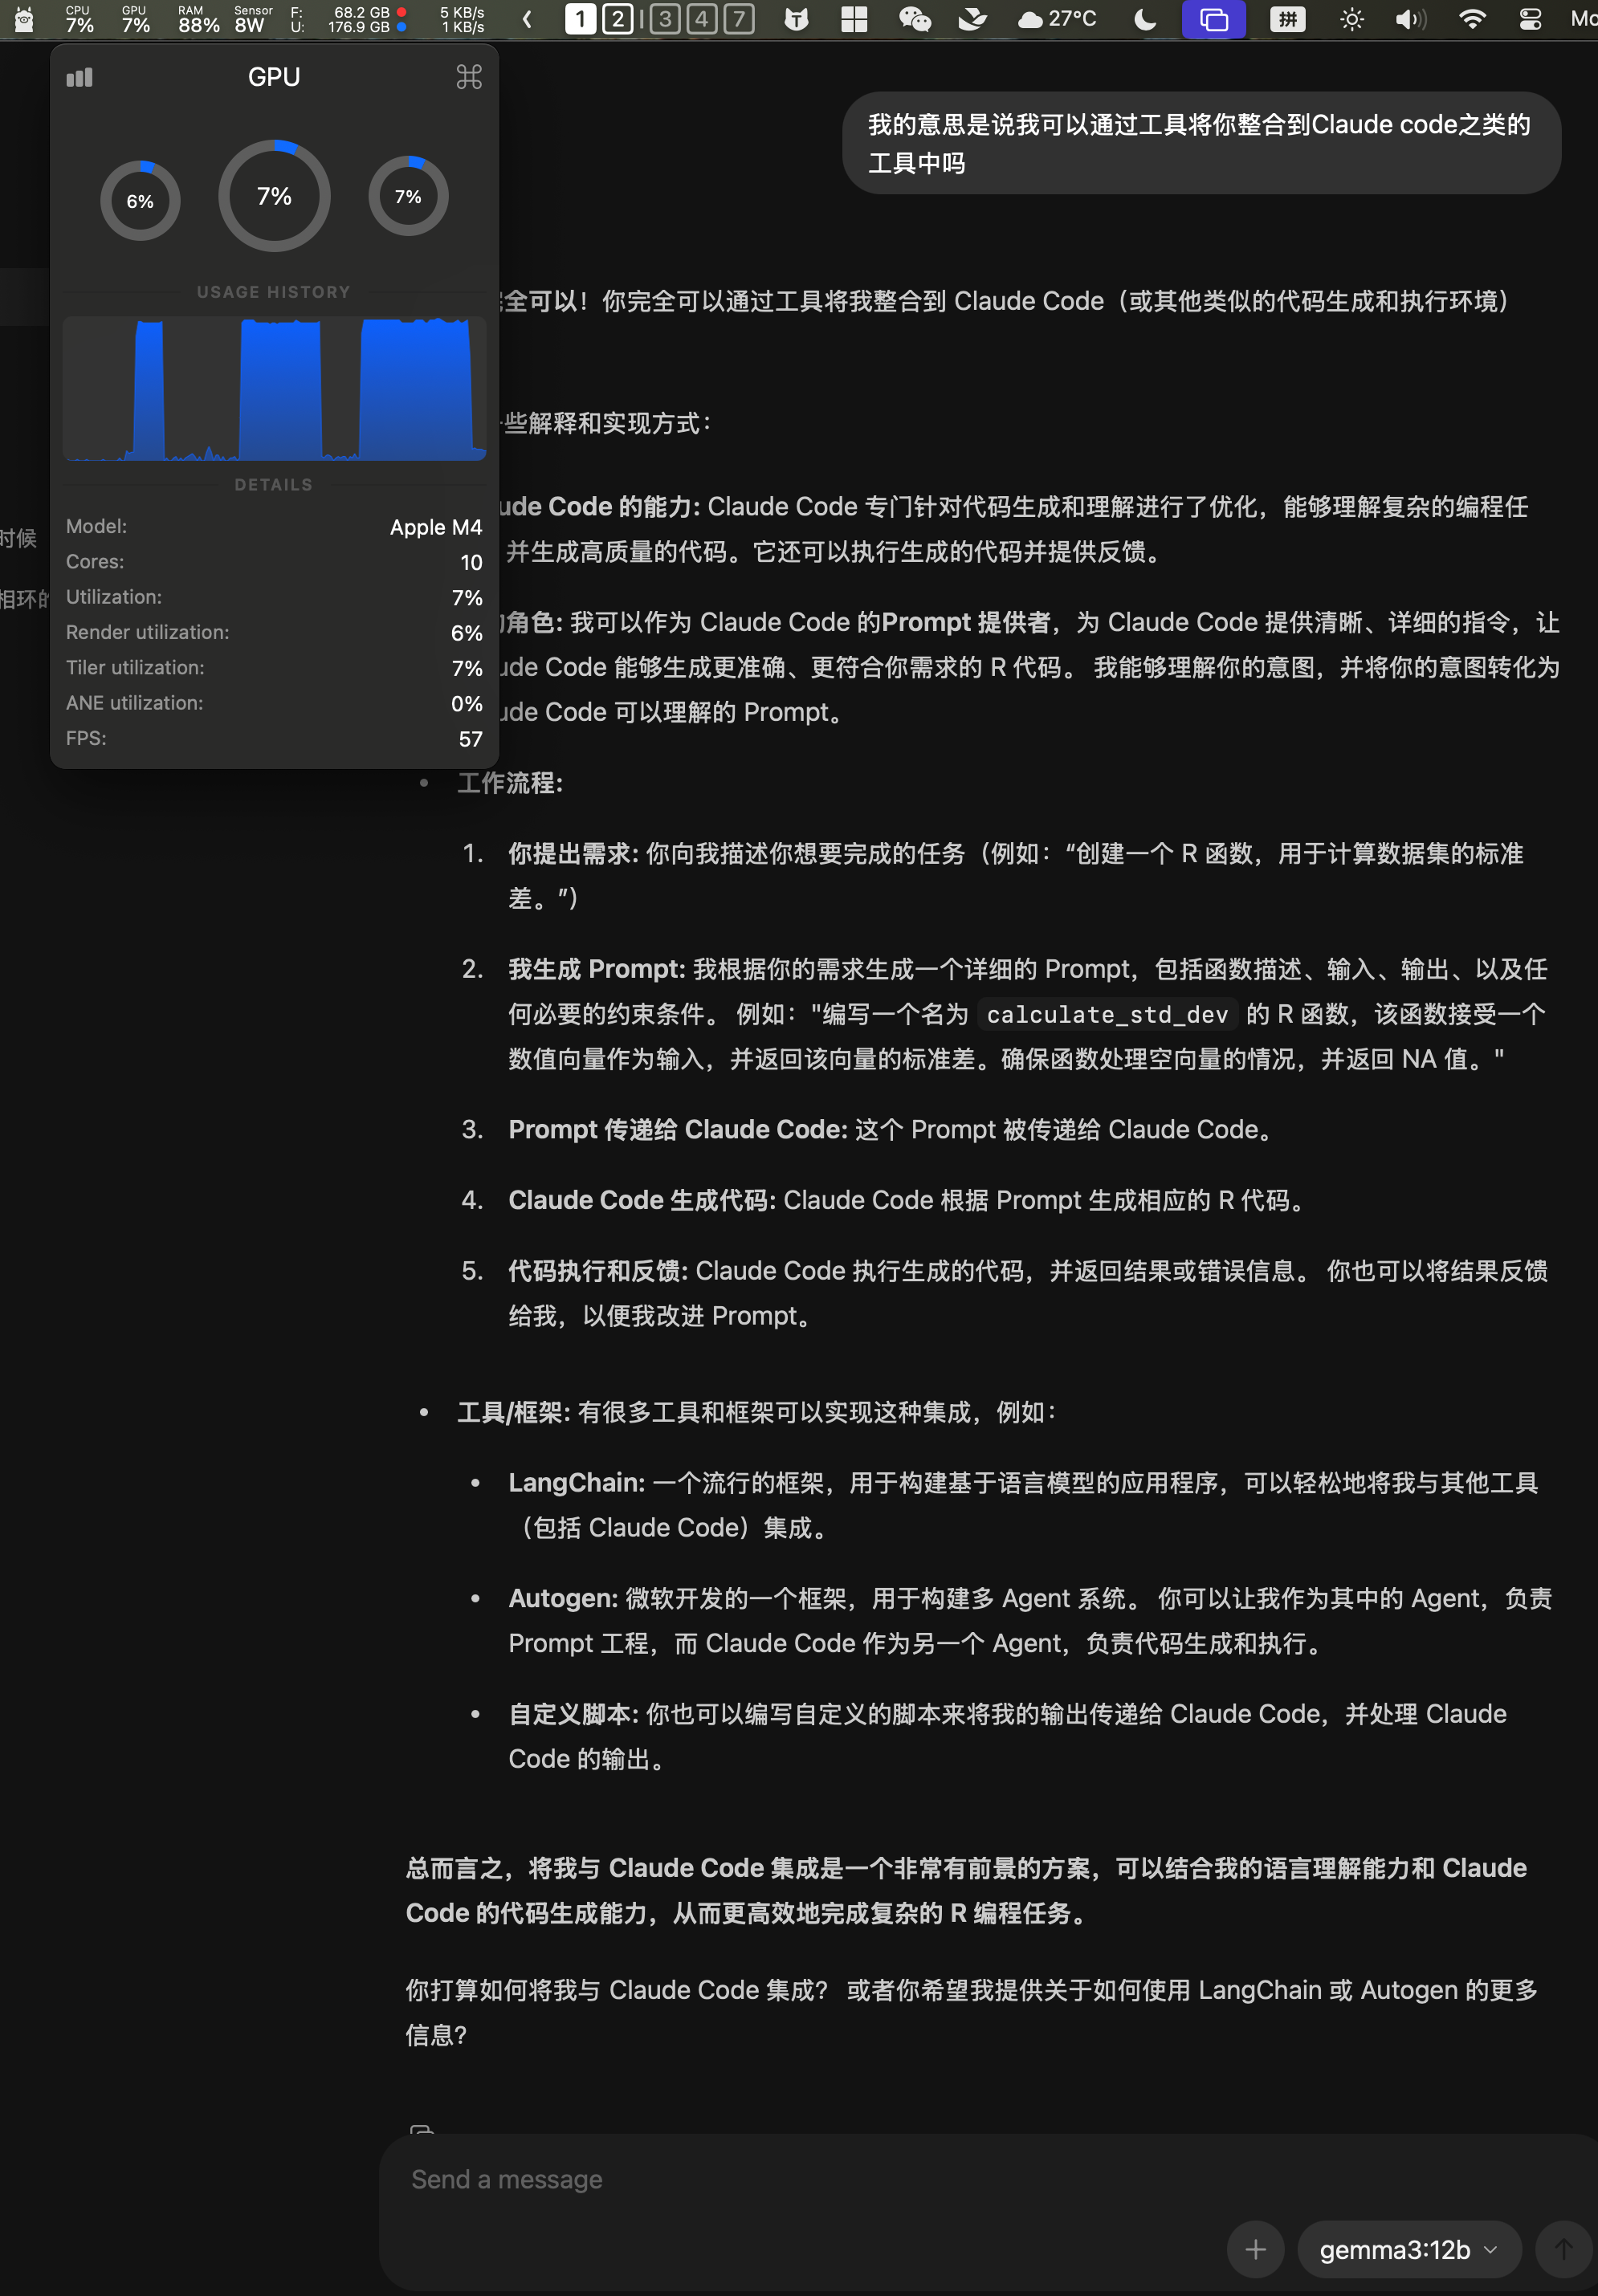
\includegraphics[width=0.72\textwidth]{figs/case_ollama.png}
    \end{column}

    \begin{column}{0.3\textwidth}
      \vspace{-3cm}
      \begin{exampleblock}{说明}
        通过 Ollama 在本地加载量化模型（图中为Gemma 4 E4B,仅4.5B参数，显存占用9.5GiB），终端直接对话。
      \end{exampleblock}
    \end{column}
  \end{columns}

\end{frame}

% --- 本地部署示例：Copilot 内网聊天 ---
\begin{frame}{本地部署示例：VS Code Copilot 本地Agent}
  \centering
  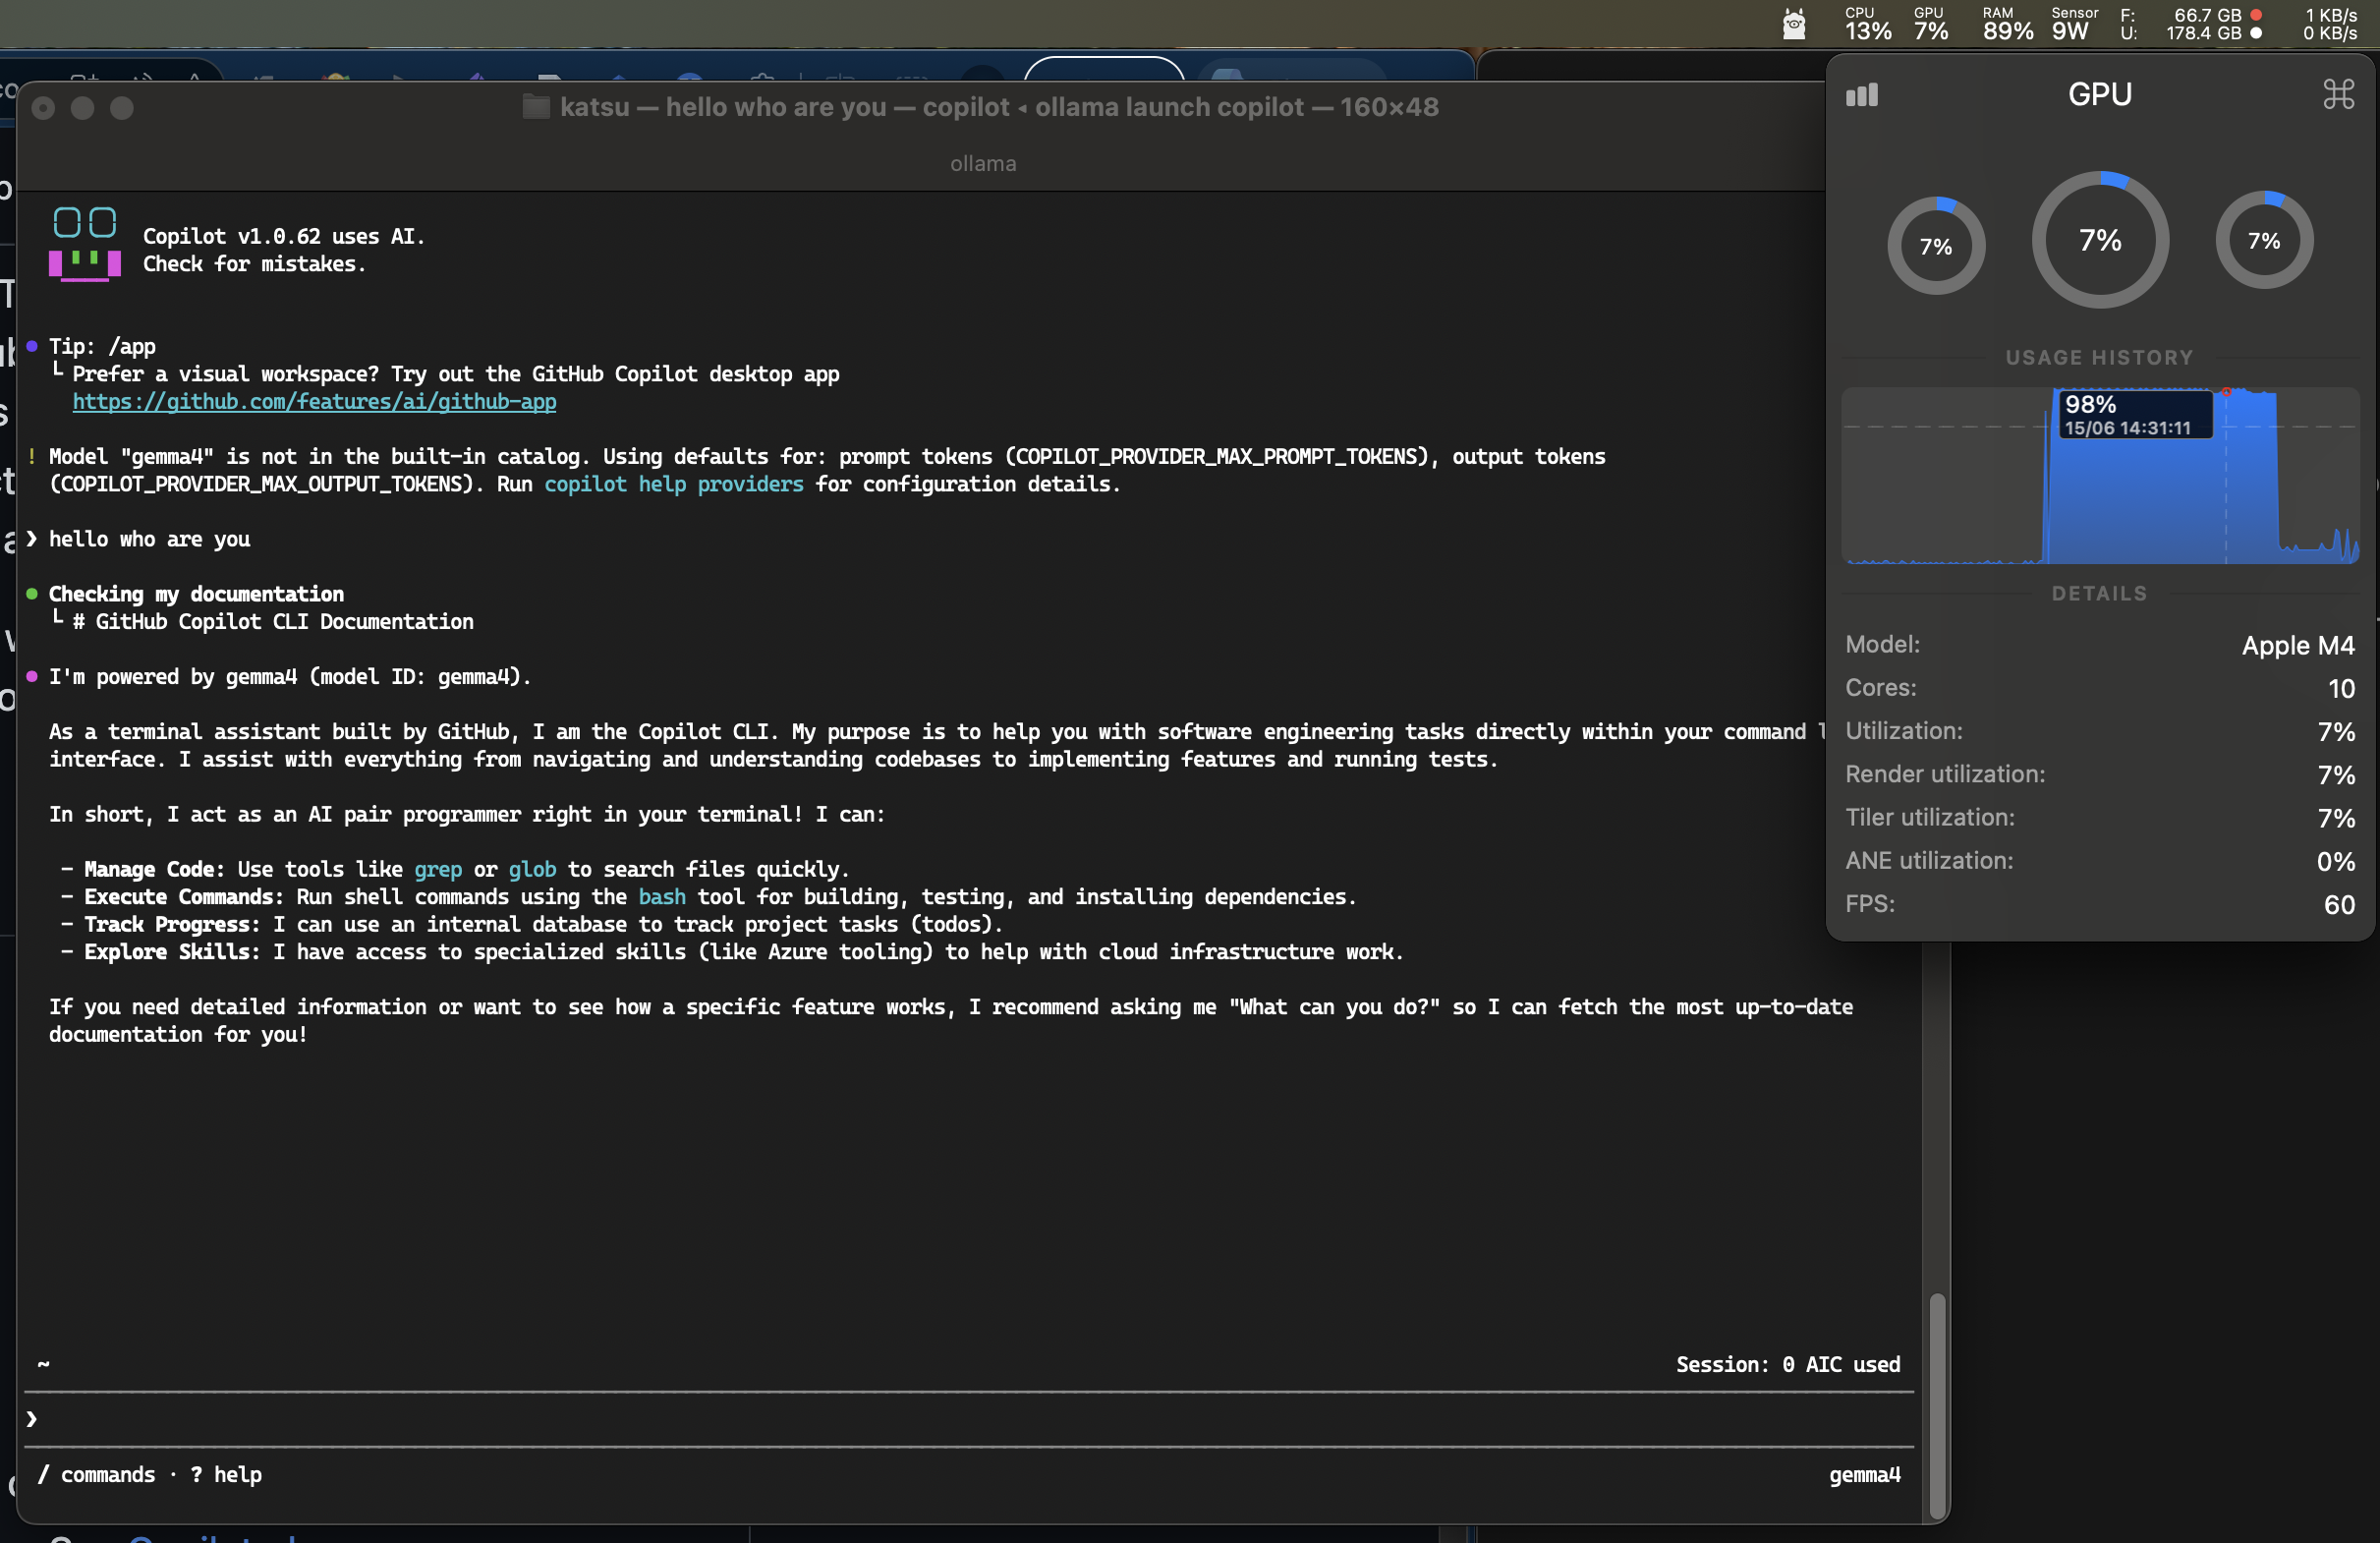
\includegraphics[width=0.62\textwidth]{figs/case_copilot.png}
  \vspace{-4pt}
  \begin{exampleblock}{说明}
    \small Agent类代码工具对接本地推理服务：途中通过 Copilot  CLI 与本地 LLM 交互.可用于完成代码生成、文档查询、日志分析等任务
  \end{exampleblock}
\end{frame}


% ================================================================
\section{总结}
% ================================================================

\begin{frame}{三大应用方向总结}
  \begin{table}
    \centering
    \begin{tabular}{l p{35mm} p{55mm}}
      \toprule
      领域 & 核心场景 & 关键价值 \\
      \midrule
      数字 IC
        & EDA 脚本、模板代码、协议解析
        & 减少重复劳动、加速设计迭代、降低查阅成本 \\
      \midrule
      模拟 IC
        & 仿真脚本、数据清洗与可视化
        & 降低小众语言门槛、自动化后处理流程 \\
      \midrule
      实验室建设
        & 新人培训、文档规范化
        & 释放指导精力、提升文档可复用性 \\
      \bottomrule
    \end{tabular}
  \end{table}

  \vspace{8pt}
  \begin{exampleblock}{核心判断}
    内网 LLM 在 IC 实验室场景中，价值不在于替代工程师的创造力，而在于消除 \textbf{重复性、事务性} 工作对创造力的挤占。
  \end{exampleblock}
\end{frame}

% ============================================
%  结束页
% ============================================
\begin{frame}[plain]
  \centering
  \vfill
  {\huge\color{ieeeBlue} 谢谢！欢迎提问}

  \vspace{20pt}
  {\large 邮箱：katsu119@foxmail.com}

  \vspace{8pt}
  {\large GitHub：github.com/katsu119}
  \vfill
\end{frame}

\end{document}
